\documentclass[runningheads]{llncs}
\usepackage{graphicx}
\usepackage{subcaption}
\usepackage[spanish]{babel}
\addto\captionsspanish{%
  \renewcommand{\tablename}{Tabla}
}
\usepackage{csquotes}
\usepackage[margin=1in]{geometry}
\usepackage{amsmath}
\usepackage{amsfonts}
\usepackage{csquotes}
\usepackage{url}
\usepackage{xurl} % Permite que las URLs largas se corten bien al final de la línea
\usepackage[hidelinks]{hyperref} % Hace que los links sean cliqueables pero sin cuadros de colores
\usepackage{inconsolata}
\usepackage{float}
\usepackage{xcolor}
\usepackage{hyperref}
\usepackage{booktabs}
\usepackage{caption}
\captionsetup[table]{skip=10pt}
\usepackage{algorithm}
\usepackage{algorithmic}
\floatname{algorithm}{Algoritmo}
\usepackage{tabularx}
\setcounter{secnumdepth}{4}
\raggedbottom
\usepackage{svg}
\usepackage[table]{xcolor}
\usepackage{pdfpages}


\begin{document}


\includepdf[pages=1]{portada/Formato-portada.pdf}


\title{GEODETECTOR: Un Pipeline Híbrido Basado en Inteligencia 
Artificial para la Detección, Clasificación y Geolocalización Automatizada de
 Letreros Turísticos en Rutas y Carreteras}
%
\titlerunning{GEODETECTOR}
% If the paper title is too long for the running head, you can set
% an abbreviated paper title here
%
\author{Felipe Córdova\inst{1}}
%
\authorrunning{F. Córdova}
% First names are abbreviated in the running head.
% If there are more than two authors, 'et al.' is used.
%
\institute{Universidad Austral de Chile, Valdivia, Chile\\
\email{\texttt{felipe.cordova@alumnos.uach.cl}}}

%
\maketitle              % typeset the header of the contribution
%

\begin{abstract}
El volumen de información presente en las rutas y carreteras rurales es vasto,
pero en gran medida invisible para los sistemas digitales actuales. Letreros
turísticos que anuncian servicios de alimentación, alojamiento y atracciones
locales permanecen fuera del alcance de las plataformas de mapeo convencionales,
ya que no han sido registrados de forma sistemática. La visión artificial
ofrece hoy las herramientas para cambiar eso. En este trabajo se propone 
GEODETECTOR, un pipeline híbrido que integra detección de letreros, 
extracción y mejoramiento de regiones de interés (ROI), reconocimiento 
de texto, clasificación semántica basada en taxonomía turística con 
evaluación de calidad informativa en niveles alto, medio y bajo, 
georreferenciación sincronizada y visualización de resultados, evaluado en condiciones reales de 
captura vehicular sobre tres rutas en la Región de Los Lagos, Chile. El 
pipeline fue evaluado sobre tres videos de entre 4 y 6 minutos capturados
bajo distintas condiciones climáticas, con 212 letreros reales de todo 
tipo determinados mediante conteo manual y procesados en cuatro configuraciones
(720p/1080p y 15/30 FPS). El modelo alcanzó valores de Precisión entre 0,77 y 0,91, 
Recall entre 0,50 y 0,74 y F1-score entre 0,61 y 0,76. El reconocimiento
de texto obtuvo un Character Error Rate (CER) entre 0,08 y 0,27 según las 
condiciones de captura. El pipeline logró interpretar y clasificar el
57,1\% de los letreros turísticos detectados. Los resultados evidencian la viabilidad del pipeline 
para detectar, interpretar y geolocalizar automáticamente letreros turísticos
en entornos reales, aportando además un dataset propio de 2.000 imágenes
etiquetadas publicado en IEEE DataPort.
\keywords{YOLO \and Deep Learning \and Computer Vision \and Georeferencing
 \and Optical Character Recognition (OCR) \and Scene Text Recognition (STR) 
 \and Transfer Learning}
\end{abstract}


\section{Introducción}
En los últimos años, los avances en visión artificial y aprendizaje
 profundo han permitido mejoras significativas en tareas de detección de 
 objetos y reconocimiento de texto en imágenes. Modelos basados en 
 arquitecturas como YOLO (You Only Look Once) han demostrado un alto
  desempeño en la detección de objetos viales como señales de tránsito, 
  vehículos y peatones en escenarios controlados y 
  semi-controlados \cite{articulo-trafico}. Sin embargo, su aplicación 
  en contextos distintos, como la detección de letreros turísticos no
   estandarizados, plantea desafíos adicionales que estos enfoques no 
   abordan directamente. Complementariamente, las técnicas modernas de 
   reconocimiento óptico de caracteres (OCR) han ampliado las capacidades
de extracción de información desde imágenes complejas, siendo ampliamente 
adoptadas en industrias como la banca \cite{ocr-banco}, compras en línea
 \cite{ocr-compras-en-linea} y en sistemas de salud, donde permiten 
 la digitalización y extracción automática de información desde informes 
 médicos \cite{ocr-salud}. No obstante, la aplicación conjunta de estas 
 tecnologías en entornos dinámicos no controlados, particularmente en 
 contextos de captura desde vehículos en movimiento, sigue representando 
 un desafío relevante en la literatura.

En escenarios de rutas y carretera, la detección y reconocimiento de 
letreros presenta múltiples dificultades técnicas. Entre ellas se incluyen
 el desenfoque por movimiento (motion blur) asociado a la velocidad del vehículo, 
 variaciones de iluminación como transiciones entre sombra y luz directa, 
 condiciones climáticas adversas y el ángulo de captura variable producto
  de la perspectiva, propias de escenarios con vehículos en 
  desplazamiento. Estos factores se agravan al aplicar OCR sobre imágenes 
  capturadas dinámicamente, donde la perspectiva variable, los reflejos 
  y el hecho de que el texto aparezca solo por fracciones de segundo
   mientras el vehículo avanza pueden elevar la tasa de error entre un 
   10\% y un 30\% \cite{mal-ocr-en-movimiento}.

En particular, los letreros artesanales de turismo rural presentan 
características adicionales que complejizan tanto su detección como 
el reconocimiento de su contenido textual. Como se ilustra en la 
Figura \ref{fig:letreros_rurales}, esta señalética presenta una alta 
variabilidad visual: letreros de madera con tipografías talladas o 
pintadas a mano, formas que van desde rectángulos convencionales hasta 
diseños circulares o figuras artesanales, materiales con deterioro 
físico visible, y en ocasiones varios letreros agrupados en un mismo 
punto compitiendo visualmente entre sí. A esto se suma el bajo 
  contraste entre el texto y el fondo en letreros de madera envejecida, 
  y la presencia de vegetación que genera oclusión parcial. Este escenario
   contrasta con las condiciones para las que la mayoría de los algoritmos
    OCR disponibles fueron diseñados: documentos impresos, facturas o 
    capturas de pantalla donde se asume resolución estable, fondo uniforme
     y texto alineado \cite{ocr-asumido}, supuestos que no se sostienen 
     en entornos rurales de captura dinámica.

%AGREGAR FIGURA
\begin{figure}[H]
    \centering
    
    \begin{subfigure}[b]{0.23\textwidth}
        \centering
        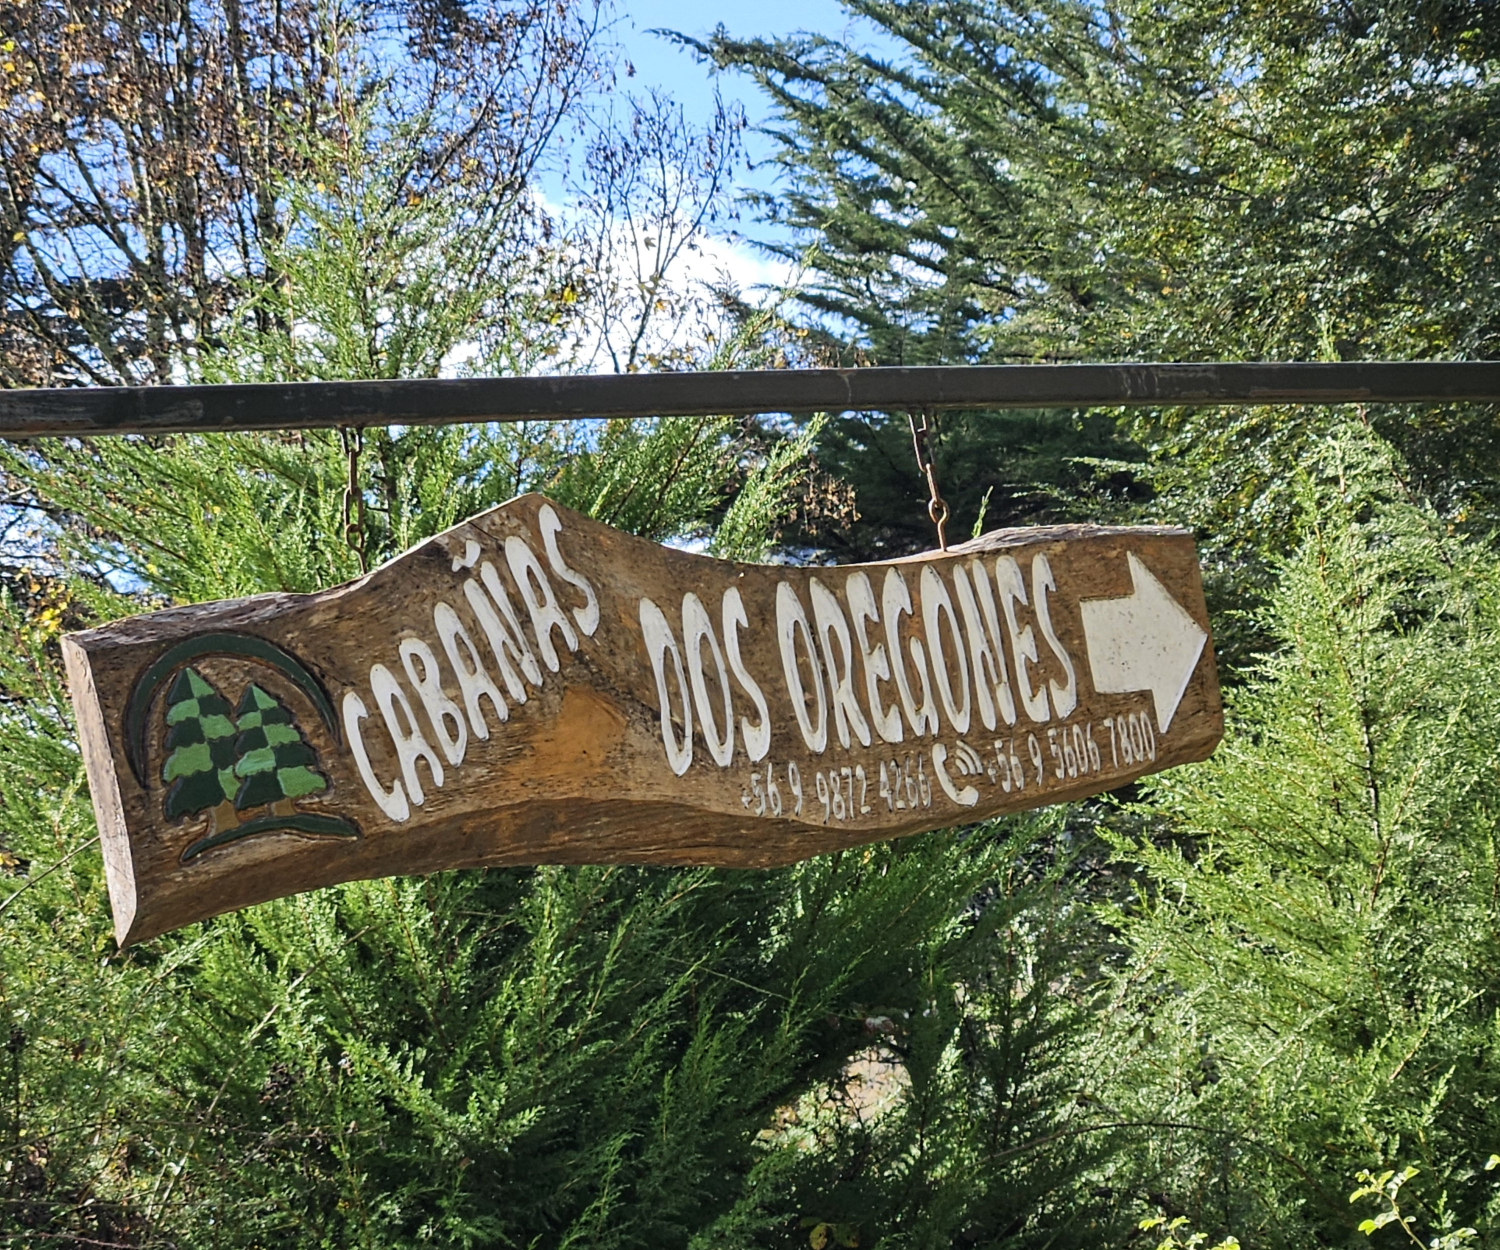
\includegraphics[width=\textwidth]{letreros/letrero2_comprimido.pdf}
    \end{subfigure}
    \hfill
    \begin{subfigure}[b]{0.23\textwidth}
        \centering
        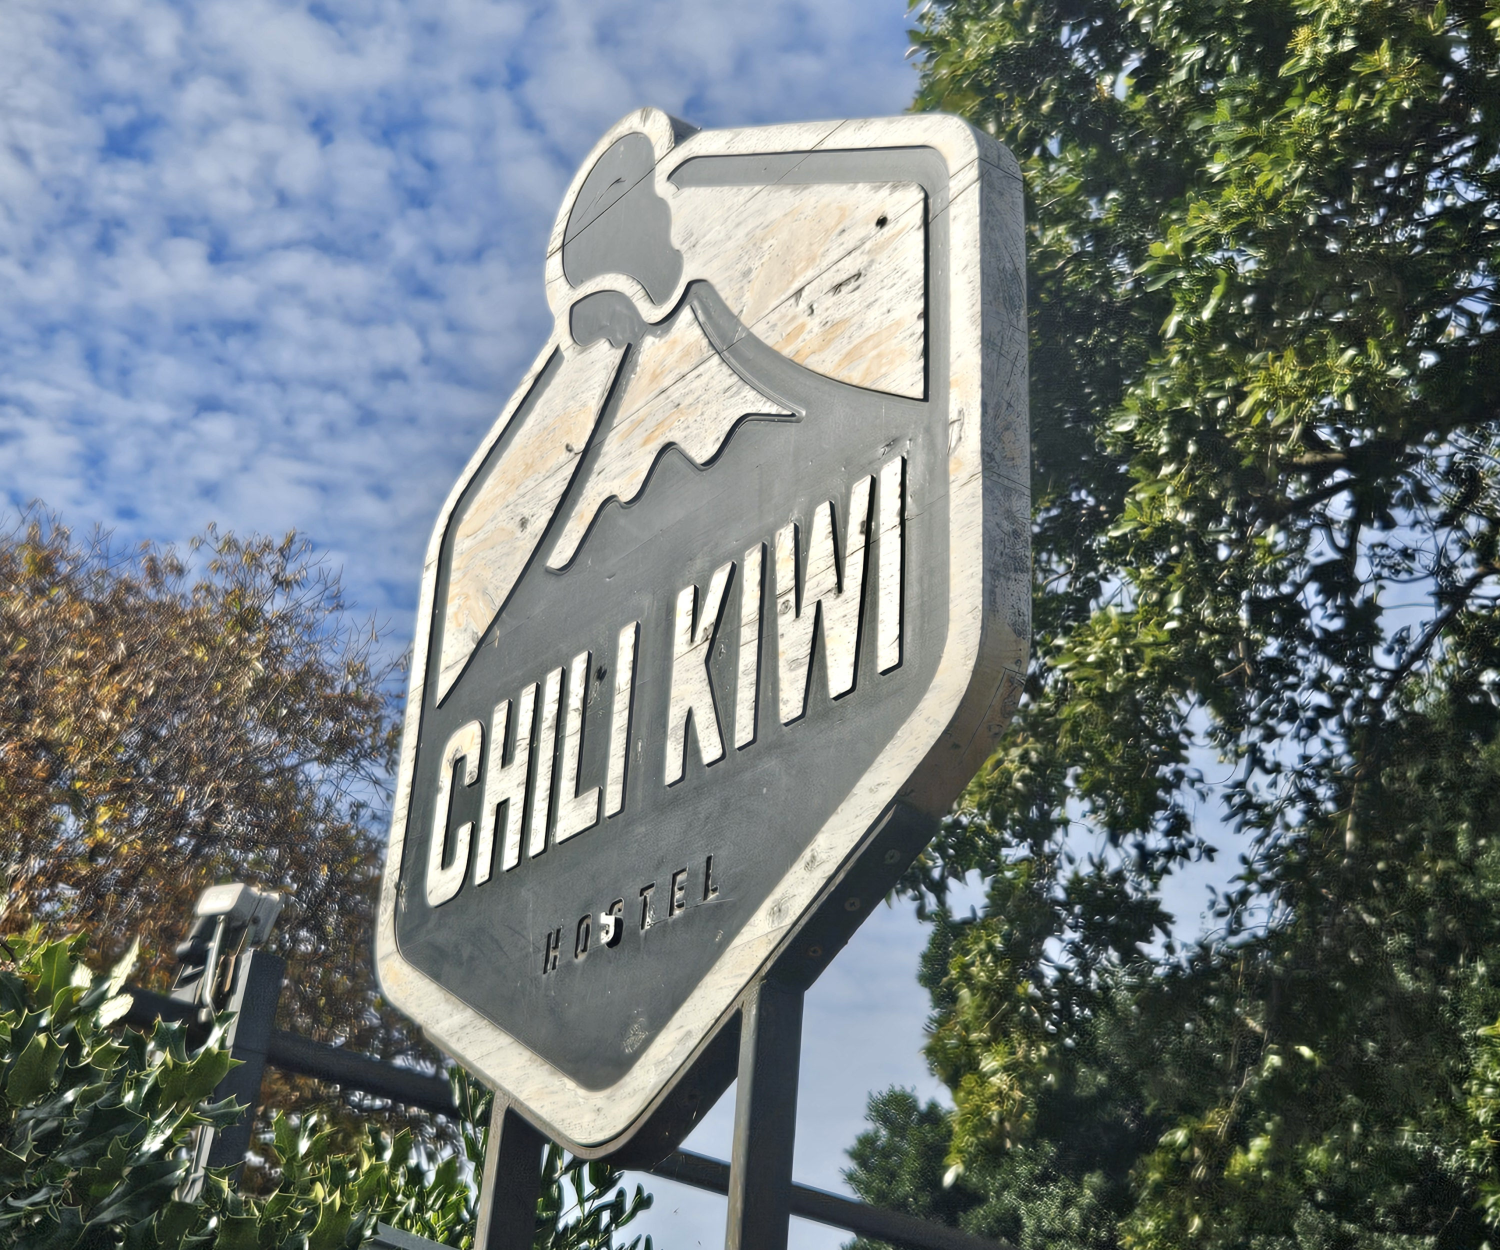
\includegraphics[width=\textwidth]{letreros/letrero3_comprimido.pdf}
    \end{subfigure}
    \hfill
    \begin{subfigure}[b]{0.23\textwidth}
        \centering
        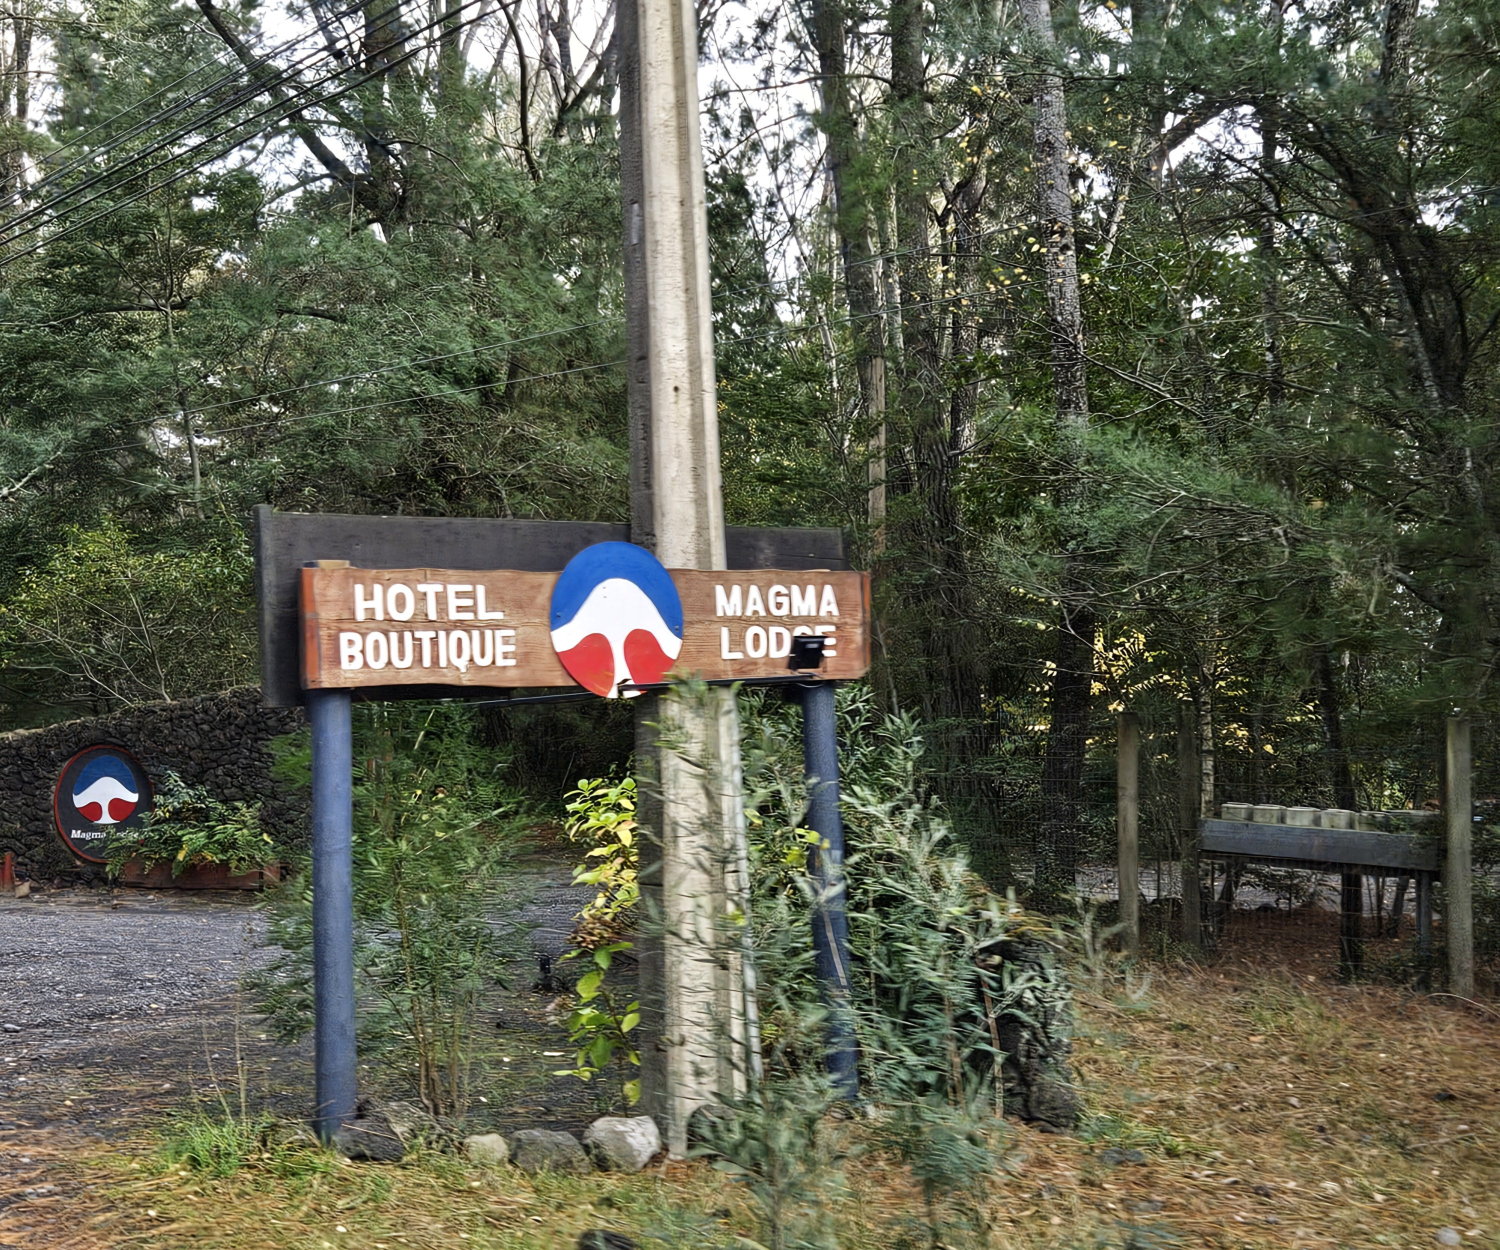
\includegraphics[width=\textwidth]{letreros/letrero10_comprimido.pdf}
    \end{subfigure}
    \hfill
    \begin{subfigure}[b]{0.23\textwidth}
        \centering
        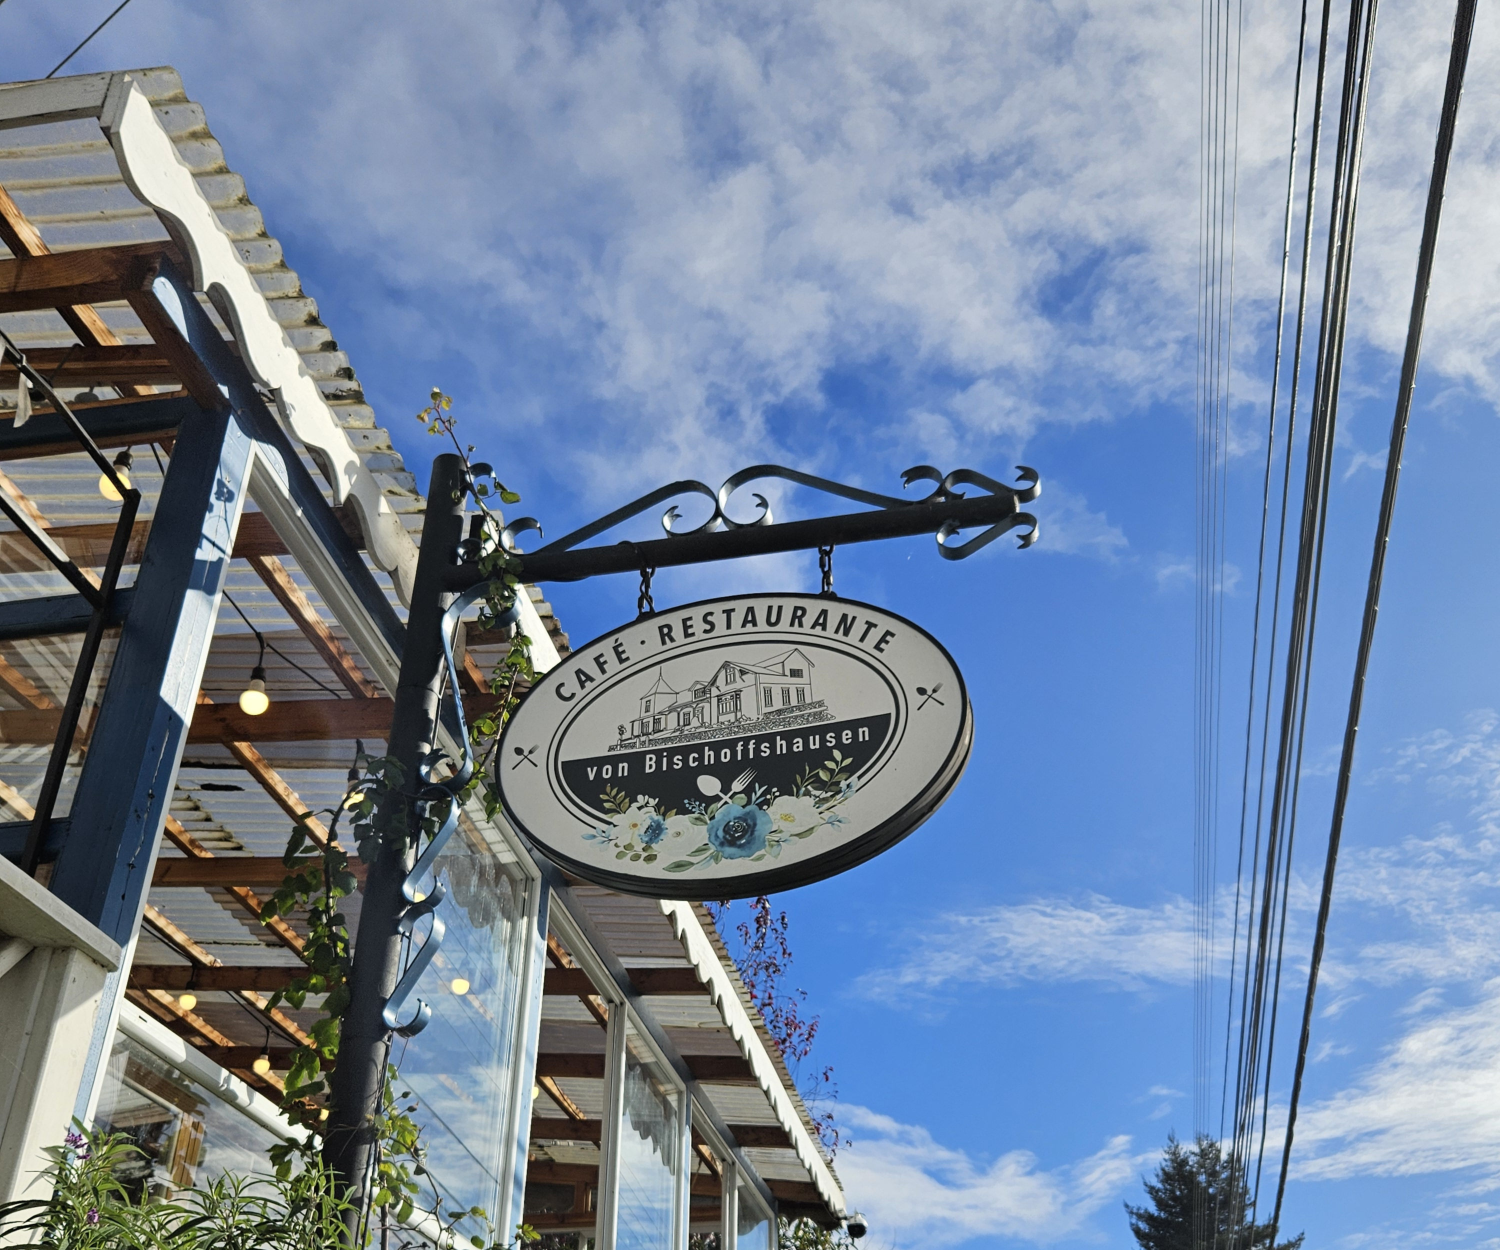
\includegraphics[width=\textwidth]{letreros/letrero5_comprimido.pdf}
    \end{subfigure}
    
    \caption{Ejemplos de letreros turísticos rurales.}
    \label{fig:letreros_rurales}
\end{figure}


A pesar de la existencia de modelos robustos para detección de objetos
 y OCR de propósito general, su integración en un pipeline capaz de
  operar de manera confiable en condiciones de captura continua, con 
  datos provenientes de video y geolocalización simultánea, ha sido 
  escasamente abordada. Los modelos de visión artificial indican dónde 
  se encuentra un objeto dentro de una imagen, pero no su ubicación 
  geográfica real \cite{roboflow-georeferencing}, lo que exige una capa 
  adicional de sincronización espacio-temporal entre el flujo de video 
  y los datos de posicionamiento GPS. Esta brecha entre detección visual,
   reconocimiento de texto y geolocalización integrada representa el 
   problema central que motiva el presente trabajo.

Un desafío adicional es la escasez de datasets representativos
para dominios específicos como la señalética turística rural, 
lo que obliga al levantamiento de datos propios en condiciones 
reales de operación \cite{dataset-no-existentes}. Los modelos 
entrenados en dominios de origen con datos abundantes tienden a 
degradar su rendimiento al aplicarse a dominios con distribuciones 
visuales distintas, fenómeno conocido como domain 
 shift (cambio de dominio) \cite{domain-shift}. Para abordar este problema, la literatura 
propone el uso de transfer learning (aprendizaje por transferencia)
\cite{transfer-learning,transfer-learning-yolo}, técnica que permite 
reutilizar los pesos de un modelo preentrenado en un dominio general 
y adaptarlo mediante fine-tuning (ajuste fino) \cite{fine-tuning} a un dominio 
específico con menor cantidad de datos, logrando resultados competitivos 
sin necesidad de entrenar desde cero.

En este trabajo se aborda el problema de la detección, 
extracción de texto y geolocalización automática de letreros 
turísticos en rutas y carreteras, considerando un escenario real de adquisición de 
datos mediante smartphones móviles en movimiento de vehículos. La 
pregunta de investigación que guía este estudio es la siguiente:

\textbf{RQ: ¿Cómo diseñar un pipeline híbrido basado en visión artificial 
y geolocalización que permita detectar y extraer información relevante 
desde letreros turísticos en condiciones dinámicas no controladas?}

Para responder a esta interrogante, se propone GEODETECTOR, 
un pipeline híbrido que integra un modelo de detección de letreros basados
 en aprendizaje supervisado, técnicas de procesamiento de regiones 
de interés, métodos de reconocimiento óptico de caracteres, 
geolocalización y sincronización. La solución es evaluada utilizando 
un dataset recolectado en condiciones reales de operación en rutas y
carreteras rurales y urbanas, lo que permite analizar su desempeño frente a los 
desafíos propios del entorno dinámico. Las principales contribuciones 
de este trabajo son las siguientes: \textbf{(i)} la construcción de un dataset 
representativo de letreros rurales y urbanos capturados en condiciones 
dinámicas reales; \textbf{(ii)} el diseño de un pipeline para la detección, 
clasificación semántica por taxonomía y geolocalización de letreros; y 
\textbf{(iii)} la evaluación del pipeline bajo condiciones no controladas, 
incluyendo un esquema de calidad de detección basado en la riqueza 
informativa de cada letrero.



\section{Trabajos Relacionados}
Esta sección revisa la literatura relevante en las áreas que sustentan el
 desarrollo de GEODETECTOR.
Se abordan cinco ejes temáticos: la detección de objetos bajo diferentes 
configuraciones de video, la detección de objetos en entornos dinámicos, 
el reconocimiento de texto en escenas naturales, 
la detección de señalética en carretera, y las limitaciones de los datasets existentes. A partir de este análisis se identifican las brechas 
que motivan las decisiones de diseño adoptadas en este trabajo.

\subsection{Detección de Objetos Bajo Diferentes Configuraciones de Video}
% buscar articulos con 2-3 nuevos. Que hablen del analisis de YOLO u otros que mezclen el procesamiento de video bajo distintos calidad de videos (resolucion del video, que funciona bien con calidad 700p), frame por segundo (yolofunciona bien con 30 frame por segundos) y el formato (mp4, etc) 
El desempeño de los modelos de detección de objetos basados en YOLO 
se ve directamente influenciado por las características del video de 
entrada, incluyendo la resolución, la frecuencia de frames por segundo 
(FPS) y el formato de captura. En el contexto de grabaciones desde 
dispositivos móviles, los formatos más comunes son \texttt{.mp4} y 
\texttt{.mov}, mientras que en sistemas de videovigilancia y cámaras 
de seguridad se utiliza frecuentemente el formato \texttt{.avi}, siendo 
este último ampliamente empleado en aplicaciones de detección de 
personas y vehículos mediante YOLO \cite{yolo-mp4-frames}. El formato 
\texttt{.mp4} destaca como el más utilizado en aplicaciones de visión 
artificial debido a su amplia compatibilidad y eficiencia en 
almacenamiento \cite{yolo-mp4-frames}. Estudios señalan que el 
procesamiento de video mediante la división en frames individuales 
permite aplicar YOLO de manera eficiente sobre cada cuadro, 
determinando tanto el instante como la ubicación del objeto detectado 
\cite{yolo-mp4-frames}. En cuanto a la resolución, se ha demostrado 
que YOLO opera de forma óptima con videos de alta resolución, logrando 
velocidades de inferencia superiores a 30 FPS con GPU, mientras que en 
CPU la velocidad puede reducirse drásticamente a entre 2 y 20 FPS 
dependiendo de la variante del modelo utilizada 
\cite{yolo-traffic-resolution}. Resoluciones inferiores a 720p pueden 
comprometer la precisión en escenarios donde los objetos de interés 
aparecen a distancia o en condiciones de baja iluminación 
\cite{yolo-traffic-resolution}. Estos antecedentes motivaron las 
decisiones de configuración adoptadas en este trabajo, donde se optó 
por capturar videos en formato \texttt{.mp4} en alta resolución (1080p)
y procesar un frame por segundo, equilibrando cobertura temporal y costo 
computacional.

\subsection{Detección de Objetos en Entornos Dinámicos}
% TODO: revisar literatura YOLO, Faster R-CNN, limitaciones en movimiento

La detección de objetos en tiempo real ha experimentado avances
significativos con la introducción de arquitecturas basadas en aprendizaje profundo. 
Entre los enfoques más influyentes se encuentran los detectores de dos 
etapas, como Faster R-CNN (Faster Region-based Convolutional Neural 
Network), que priorizan la precisión mediante la generación de 
propuestas de región \cite{rnn-faster}, y los detectores de una etapa, 
como la familia YOLO, que privilegian la velocidad de inferencia. En el 
contexto de aplicaciones vehiculares, YOLO ha demostrado ser especialmente
adecuado por su capacidad de procesar frames en tiempo 
real \cite{yolo-vehiculos}. Sin embargo, al evaluar estos modelos bajo 
condiciones de degradación visual como niebla, lluvia, nieve y desenfoque
por movimiento se ha observado una caída significativa en las métricas de detección 
\cite{yolo-escenarios-naturales}. Estudios comparativos indican que, si 
bien YOLO supera a Faster R-CNN en velocidad, ambos modelos presentan 
limitaciones cuando el dominio de captura difiere del dataset de 
entrenamiento \cite{comparacion-yolo-rnn}. Estas limitaciones motivan el
desarrollo de pipelines especializados para dominios específicos como la 
captura vehicular en rutas rurales.

\subsection{Reconocimiento de Texto en Escenas Naturales}
% TODO: OCR, scene text recognition, problemas en entornos no controlados, escribir las dificultades el OCR, velocidad, angulo, como lo ha enfrentado la gente
El reconocimiento de texto en escenas naturales conocido como Scene 
Text Recognition (STR) \cite{soni2025performance} difiere 
fundamentalmente del OCR tradicional, que opera bajo supuestos de entornos 
controlados como documentos impresos, facturas o capturas de pantalla. En 
escenas al aire libre, el texto aparece con fondos complejos, tipografías 
variables, orientaciones no horizontales y condiciones de iluminación 
heterogéneas. La captura desde vehículos en movimiento introduce desafíos 
adicionales: el desenfoque por movimiento (motion blur), el ángulo de captura 
variable y la aparición del texto por fracciones de segundo dificultan la 
extracción confiable de información \cite{problemas-ocr-movimiento}. La 
comunidad ha respondido a estos desafíos mediante arquitecturas basadas en 
redes convolucionales y modelos de atención, logrando avances en el 
reconocimiento de texto curvo, rotado y parcialmente ocluido \cite{ocr-curvo}.
Sin embargo, estas soluciones han sido evaluadas principalmente en datasets
 de texto en inglés con letreros impresos de alta calidad, sin contemplar la 
 variabilidad tipográfica y material propia de señalética artesanal en rutas 
 rurales. Esta brecha justifica la incorporación de etapas de validación 
 adicionales en el pipeline propuesto.



\subsection{Detección de Señalética en Carretera}
% TODO: traffic signs vs letreros rurales (gap importante), principalmente transito, lo que tiene que ver tu turismo no esta tan marcado
La detección de señales viales ha sido ampliamente estudiada en el 
contexto de sistemas de transporte inteligente y conducción autónoma. 
Datasets como TT-100K (Tsinghua-Tencent 100K) \cite{TT100K-Dataset}, 
GTSDB (German Traffic Sign Detection Dataset) \cite{gtsdb-dataset} y 
variantes del COCO (Common Objects in Context) \cite{coco-microsoft} 
han permitido entrenar modelos de alta precisión para señales reguladas 
como límites de velocidad, señales de pare y semáforos bajo condiciones 
de captura estandarizadas \cite{letreros-transito-pare-semaforo-1}. 
Sin embargo, la gran mayoría de estos trabajos se concentra en señalética
oficial de tránsito, que posee características visuales homogéneas: 
formas geométricas definidas, colores estandarizados y tipografías 
reguladas \cite{articulo-trafico}. La señalética turística rural, en 
cambio, presenta una variabilidad visual sustancialmente mayor: materiales
 artesanales como madera o metal oxidado, tipografías no estandarizadas, 
 distintos tamaños y estados de deterioro, y ausencia de normas de diseño 
 comunes \cite{senales-rurales}. Esta brecha entre la señalética de 
 tránsito ampliamente cubierta por la literatura y los letreros turísticos
  rurales representa un área escasamente explorada, que el presente
   trabajo aborda directamente.

\subsection{Limitaciones de Datasets Existentes}
% TODO: COCO, ICDAR, ausencia de escenarios rurales dinámicos, pero no tiene la realidad local, no son carteles en español, no son de madera
Los datasets más utilizados en visión artificial, como
COCO \cite{coco-microsoft}, han sido fundamentales para el avance del 
campo. COCO incluye 80 categorías \cite{80-clases-yolo} de objetos 
cotidianos orientadas a escenas urbanas, sin contemplar 
categorías específicas de señalética turística o letreros 
artesanales \cite{ultralytics_datasets_detect}. Por su parte, los 
datasets de referencia para OCR y STR, como ICDAR 2015 \cite{icdar}, 
están compuestos principalmente por texto en inglés 
capturado en entornos urbanos de países desarrollados, en condiciones 
de iluminación aceptable y con letreros impresos de alta 
calidad. Estos datasets no representan la realidad local de rutas rurales
latinoamericanas, donde los letreros turísticos están 
frecuentemente escritos en español, fabricados con materiales rústicos
 como madera o pintura artesanal, y capturados bajo 
condiciones climáticas y de iluminación variables \cite{senales-rurales}.
Esta ausencia de datos representativos para el dominio
objetivo obliga al levantamiento de datasets propios, validando la 
decisión metodológica de recolección de datos en terreno 
adoptada en este trabajo.


% =====================================================
\section{Metodología}
En esta sección se describe la estructura metodológica adoptada para el 
diseño e implementación de GEODETECTOR. El pipeline fue construido como 
una secuencia de etapas ejecutadas localmente, donde cada componente 
resuelve una parte específica del problema: desde la adquisición de datos 
hasta la visualización georreferenciada de los resultados. Las decisiones 
de diseño fueron guiadas por las limitaciones identificadas en la 
literatura y por las condiciones reales del entorno de captura.

\subsection{Descripción General del Pipeline}
El pipeline se organiza en dos etapas, tal como se ilustra 
en la Figura~\ref{fig:pipeline}. La \textbf{Etapa 1} se orienta a la construcción y validación del modelo de inteligencia artificial, abarcando la construcción del 
dataset, su división en subconjuntos de entrenamiento, validación y 
prueba, el entrenamiento del modelo de detección de letreros, y las 
pruebas del modelo resultante. La \textbf{Etapa 2} 
corresponde a la implementación del modelo en un contexto real de 
captura vehicular, integrando la captura de video y geolocalización, 
la detección de letreros mediante el 
modelo entrenado, la sincronización de ambas fuentes, la extracción 
de ROI (Region Of Interest) y procesamiento de imagen, el reconocimiento 
de texto mediante OCR, la identificación y categorización 
de las detecciones, y finalmente la visualización de los resultados en 
un mapa interactivo.

\begin{figure}[H]
    \centering
    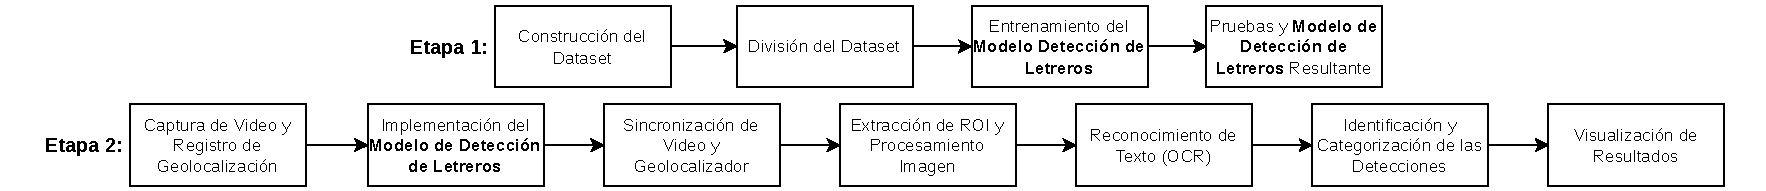
\includegraphics[width=1\textwidth]{images/pipeline-actualizado.pdf}
    \caption{Diagrama del pipeline de construcción e implementación 
    del modelo de detección de letreros.}
    \label{fig:pipeline}
\end{figure}

Como punto de partida, se evaluó la viabilidad de utilizar el modelo 
YOLO con sus clases predefinidas para la detección de objetos. El 
modelo base de YOLO incluye 80 clases \cite{80-clases-yolo,ultralytics_datasets_detect} 
orientadas a objetos comunes, tales como \textit{car}, \textit{bus}, 
\textit{truck}, \textit{person}, \textit{sports ball} y 
\textit{traffic light}, entre otras, donde esta última correspondía a 
la categoría más ``cercana'' al dominio objetivo. Sin embargo, como se 
ilustra en la Figura~\ref{fig:semaforos}, al aplicar esta clase sobre 
imágenes que contenían letreros junto a un semáforo, el modelo 
detectó exclusivamente este último, ignorando por completo la 
señalética de interés. Este resultado permite evidenciar que los modelos de 
propósito general no son adecuados para el dominio objetivo, 
justificando la necesidad de entrenar un modelo propio con datos 
representativos del problema.

\begin{figure}[H]
    \centering
    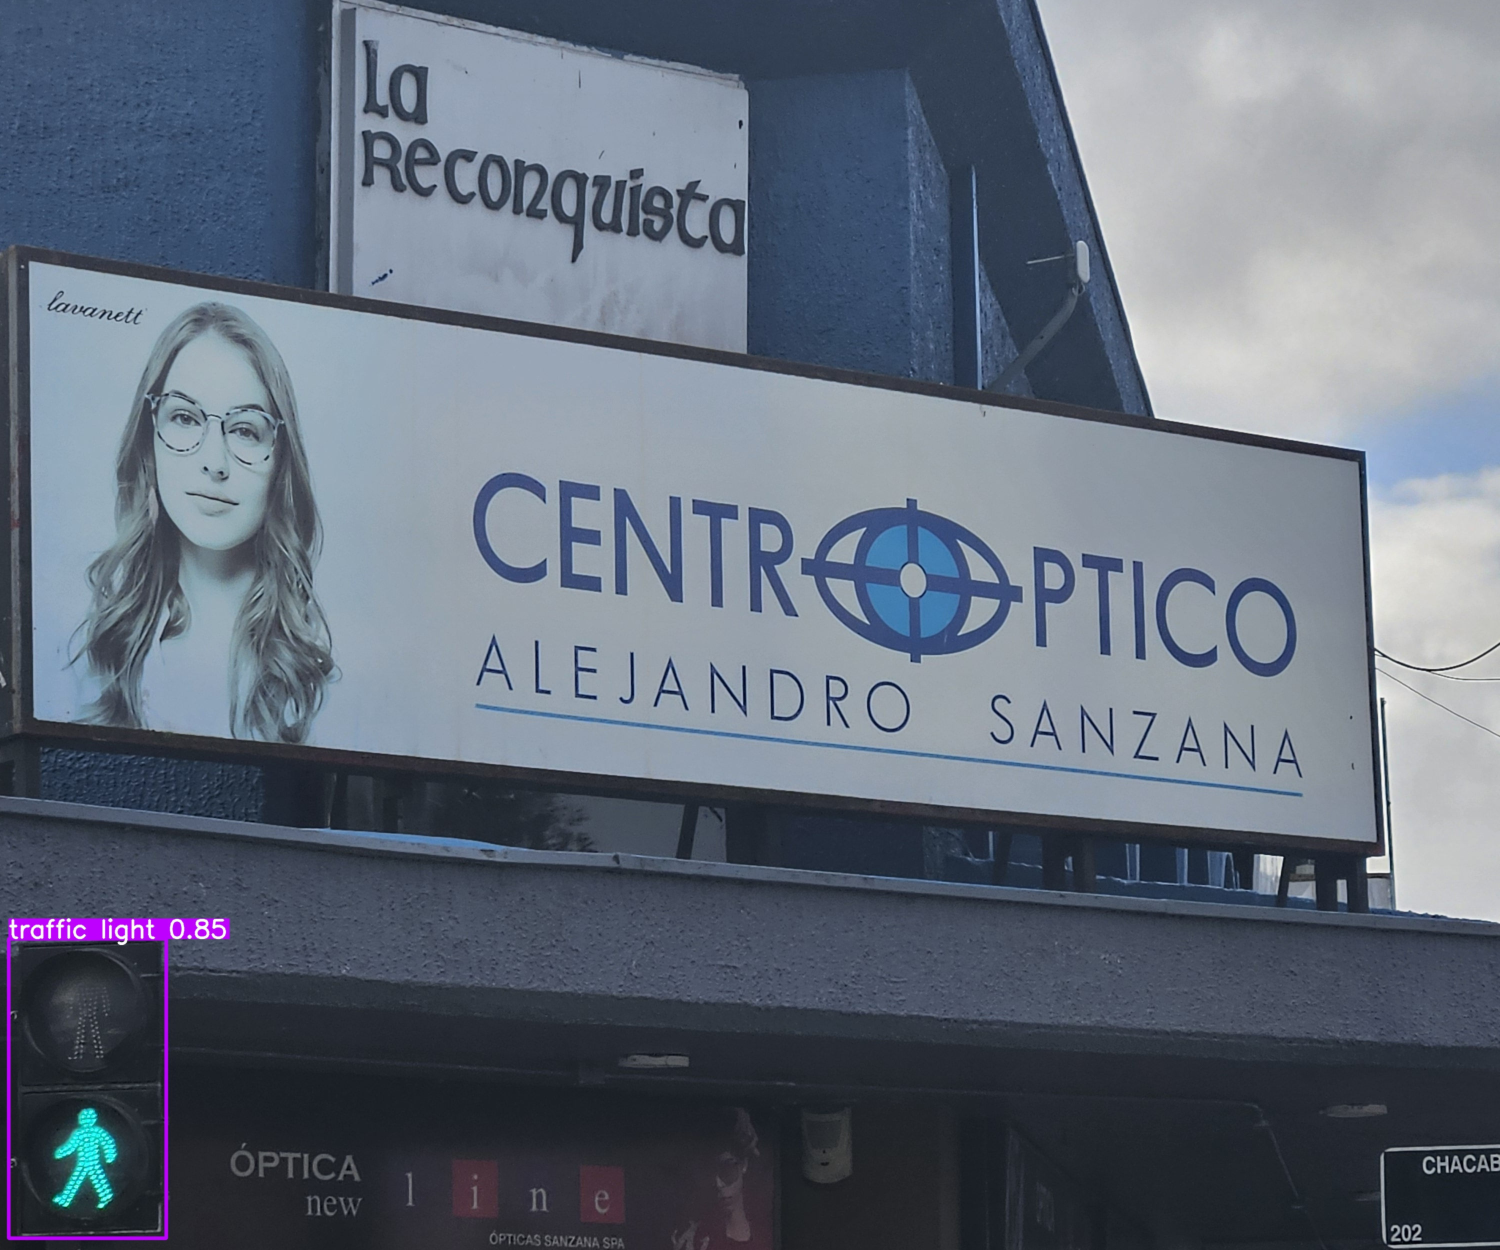
\includegraphics[width=0.23\linewidth]{semaforos/semaforo1_comprimido.pdf}
    \caption{Ejemplo de detección de la clase \textit{traffic light} (semáforo) con
     una confianza de 0,85, donde el modelo identifica correctamente el
      semáforo e ignora los letreros presentes en la escena.}
    \label{fig:semaforos}
\end{figure}


\subsection{Etapa 1: Construcción del Modelo de Detección de Letreros}
En esta subsección se describen los pasos necesarios para construir el 
modelo de detección de letreros utilizado en GEODETECTOR, siguiendo la 
secuencia definida en la Etapa 1 de la Figura~\ref{fig:pipeline}. El 
proceso abarca desde la recolección y construcción del dataset, su 
división en subconjuntos de entrenamiento, validación y prueba, el 
entrenamiento del modelo mediante transfer learning y fine-tuning, 
hasta las pruebas y evaluación del modelo resultante.

\subsubsection{Construcción del Dataset}
% Adquisición, condiciones, anotación, clases, decir que recorri regiones de chile para capturar fotos, son 2000, el dispositivo usado s23, resolucion, decir que las fotos fueron caminando, 
La construcción del dataset constituye la base del pipeline, dado que
 la calidad y diversidad de los datos de entrenamiento determinan 
 directamente el desempeño del
modelo de detección de letreros. Para garantizar representatividad, se realizaron 
recorridos por cinco regiones de Chile y zonas limítrofes de Argentina, 
capturando imágenes
de letreros en contextos variados: zonas urbanas, rutas rurales, áreas 
turísticas y localidades de distinto tamaño. Las regiones cubiertas fueron La Araucanía,
Los Ríos, Los Lagos, O'Higgins y El Maule, complementadas con capturas realizadas en territorio argentino.
El proceso de recolección se extendió desde el 8 de enero de 2025 hasta el 24 de septiembre de 2025, contemplando condiciones heterogéneas de 
iluminación, distancia, ángulo de captura y estado de conservación de la señalética.

Las imágenes fueron capturadas caminando por los distintos sectores 
con un smartphone Samsung
Galaxy S23, lo que permitió obtener capturas de alta calidad a distancias y ángulos
representativos de un recorrido real. La distribución geográfica de las capturas se resume en la
Tabla~\ref{tab:distribucion_imagenes}, que detalla la cantidad de imágenes recolectadas por región.


\begin{table}[H]
\centering
\caption{Distribución geográfica de las imágenes recolectadas.}
\label{tab:distribucion_imagenes}

\begin{tabular}{|c|>{\centering\arraybackslash}p{7cm}|c|}
\hline
\rowcolor{gray!20}
\textbf{Región} & \textbf{Localidades principales} & \textbf{Cantidad de imágenes} \\
\hline
La Araucanía & Pucón, Villarrica, Caburgua, Licanray, Loncoche & 979 \\
\hline
Los Lagos & Puerto Montt, Frutillar, Calbuco, Puerto Varas & 542 \\
\hline
Los Ríos & Valdivia, Panguipulli, Lago Ranco, Lanco & 467 \\
\hline
O'Higgins & Quinta de Tilcoco, Rancagua & 7 \\
\hline
El Maule & Colbún, San Clemente & 2 \\
\hline
Argentina & San Carlos de Bariloche & 3 \\
\hline
\end{tabular}

\end{table}

El dataset resultante comprende 2.000 imágenes, etiquetadas manualmente 
mediante la herramienta Label Studio \cite{labelstudio2026}, donde cada 
letrero visible fue etiquetado encerrando su área con un \textit{bounding 
box} (caja delimitadora). Cada etiqueta es almacenada en un archivo TXT 
con el mismo nombre que la imagen correspondiente, en el formato estándar 
de YOLO \cite{ultralytics_datasets_detect}, donde cada línea contiene los campos \texttt{class x\_center 
y\_center width height}, representando respectivamente la clase del 
objeto, las coordenadas del centro del bounding box y sus dimensiones, 
todos normalizados en el rango $[0, 1]$ respecto a las dimensiones de 
la imagen. Dado que el dataset contempla una única clase, todos los 
letreros fueron etiquetados con la clase \texttt{0}, es decir, \texttt{signboard} (letrero). 
Paralelamente, se desarrolló un script en Python \cite{python2026} que 
extrajo automáticamente la metadata de cada imagen, incluyendo timestamp 
de captura, dimensiones en píxeles y extensión de archivo, información 
que junto al nombre del archivo y la etiqueta correspondiente fue 
almacenada en un archivo Excel para su trazabilidad. Como mecanismo de 
protección de privacidad, se utilizó GIMP \cite{gimp2026} para aplicar 
un efecto de desenfoque sobre rostros de personas, patentes de vehículos, códigos QR y números de teléfono visibles en los letreros que aparecían en las 
imágenes. Adicionalmente, dado que la metadata ya había sido extraída y 
preservada en el Excel, se empleó la misma herramienta para eliminar la 
metadata embebida en cada archivo de imagen, lo que permitió reducir 
considerablemente el tamaño total del dataset en disco. El dataset 
completo fue publicado en IEEE DataPort \cite{ieee-dataset}, donde se 
encuentra disponible públicamente para su utilización por la comunidad 
científica, con el fin de respaldar y fomentar futuras investigaciones 
en el área. El repositorio incluye las 2.000 imágenes (8,26 GB), los 
archivos de etiquetas en formato TXT compatible con YOLO (529,88 KB), 
y los archivos de metadata en formato CSV y Excel (294 KB y 199,5 KB 
respectivamente).

\subsubsection{División del Dataset}
% train / validation / test
Las 2.000 imágenes y sus etiquetas correspondientes fueron divididas 
en tres subconjuntos siguiendo una proporción estándar en la literatura 
para tareas de detección de objetos: 70\% para entrenamiento, 15\% para 
validación y 15\% para prueba, resultando en 1.400, 300 y 300 imágenes 
respectivamente. La asignación de cada imagen a su subconjunto fue 
realizada de forma completamente aleatoria, con el objetivo de garantizar 
una distribución representativa de las distintas condiciones de captura 
presentes en el dataset. Cada archivo de etiqueta en formato TXT comparte 
el mismo nombre que su imagen correspondiente, organizándose en una 
estructura de carpetas paralela a la de las imágenes, donde la carpeta 
\texttt{images/} y la carpeta \texttt{labels/} contienen cada una los 
tres subconjuntos \texttt{train/}, \texttt{val/} y \texttt{test/}.

\subsubsection{Entrenamiento del Modelo Detección de Letreros}
% 50 epocas, pseudocodigo, etc
Para la detección de letreros se empleó YOLO11 \cite{yolo11_ultralytics}, 
seleccionando la variante medium (\texttt{yolo11m.pt}) tras pruebas 
comparativas con todas las variantes disponibles. Los modelos large y 
extra-large presentaron señales de \textit{overfitting} (sobreajuste), 
ya que su arquitectura de mayor complejidad requiere volúmenes de datos 
significativamente superiores a las 2.000 imágenes disponibles para 
alcanzar una buena generalización, mientras que nano y small mostraron 
capacidad de representación insuficiente. La variante medium, con 20,1 
millones de parámetros, fue seleccionada por equilibrar de mejor manera 
la capacidad de representación y generalización para el tamaño del 
dataset construido. Su desempeño base se mide mediante el 
mAP\textsubscript{val}\textsuperscript{50-95} \cite{yolo11_ultralytics}, 
métrica estándar en detección de objetos que evalúa qué tan bien el 
modelo localiza y clasifica objetos, promediando la precisión a distintos 
niveles de exigencia en la superposición entre el recuadro detectado y 
el recuadro real: un valor de 0 indica ausencia total de detecciones 
correctas, mientras que 100 representa una detección perfecta. La 
variante medium alcanza un valor de 51,5 sobre el dataset de referencia 
COCO \cite{coco-microsoft}, lo que refleja un desempeño sólido 
considerando la alta diversidad de objetos que ese benchmark contempla.

Se optó por una estrategia de transfer learning \cite{transfer-learning}, 
reutilizando los pesos preentrenados de \texttt{yolo11m.pt} y 
ajustándolos mediante fine-tuning \cite{fine-tuning} sobre el dataset 
propio. El entrenamiento se configuró con 50 épocas máximas y tamaño 
de imagen de $640 \times 640$ píxeles, tal como indica la documentación 
oficial de YOLO11 \cite{yolo11_ultralytics}. Si bien las imágenes del 
dataset presentan dimensiones superiores, YOLO aplica internamente una 
técnica de \textit{letterboxing} \cite{letterbox-yolo} que redimensiona 
la imagen preservando su relación de aspecto y rellena con padding los 
bordes restantes hasta alcanzar las dimensiones configuradas, por lo que 
no se requiere redimensionamiento manual previo. Adicionalmente, se 
configuró \textit{early stopping} (parada temprana) con una paciencia de 
5 épocas para evitar overfitting. Esto implica que el entrenamiento
 se detiene automáticamente si durante 5 épocas consecutivas no se observa
  una mejora en la métrica de validación utilizada para evaluar el desempeño del modelo.

\subsubsection{Pruebas y Modelo de Detección de Letreros Resultante}
Una vez finalizado el entrenamiento, se evaluó el modelo utilizando el 
conjunto de prueba compuesto por las 300 imágenes no vistas durante el 
aprendizaje, garantizando así una medición objetiva de su capacidad de 
generalización. El modelo completó las 50 épocas de entrenamiento 
alcanzando resultados sobresalientes. La Figura~\ref{fig:results_mosaico} 
presenta la evolución de las curvas de pérdida y métricas a lo largo 
del entrenamiento, donde es posible observar que tanto las pérdidas de 
entrenamiento (\texttt{train/box\_loss}, \texttt{train/cls\_loss},
\texttt{train/dfl\_loss}) como las de validación (\texttt{val/box\_loss},
\texttt{val/cls\_loss}, \texttt{val/dfl\_loss}) 
mostraron un descenso constante y sostenido durante todo el proceso, 
sin presentar divergencia entre ambas curvas, lo que confirma la 
ausencia de overfitting.

\begin{figure}[H]
    \centering
    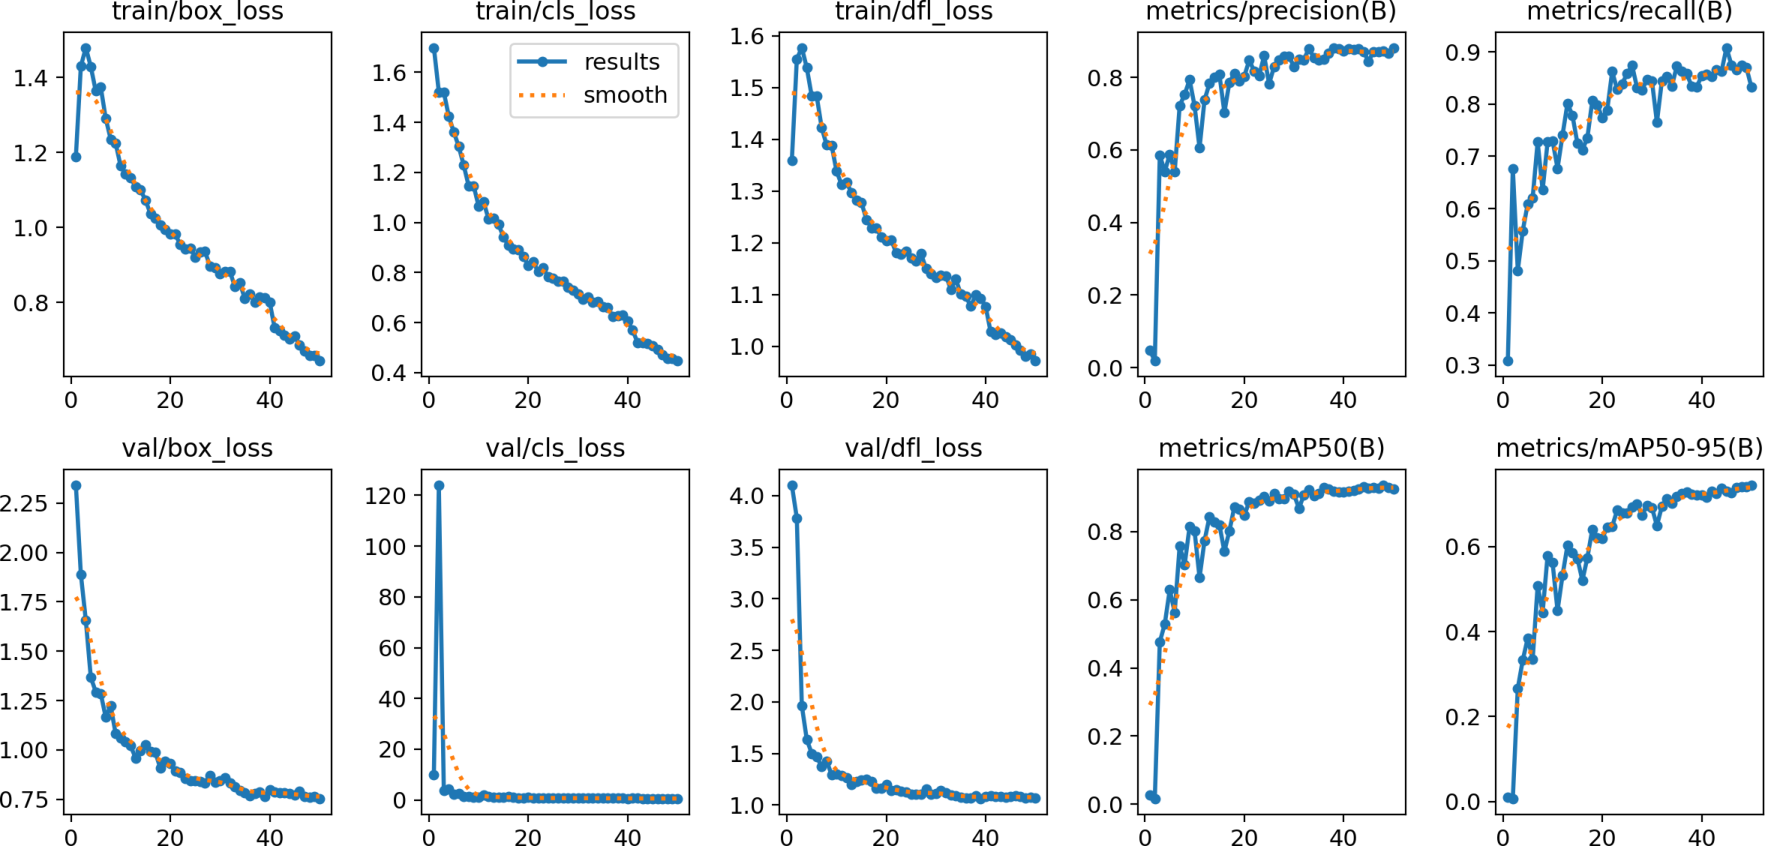
\includegraphics[width=1\textwidth]{images/results.pdf}
    \caption{Curvas de pérdida y métricas durante el entrenamiento y validación del modelo YOLO11m.}
    \label{fig:results_mosaico}
\end{figure}


Los valores finales obtenidos al término del entrenamiento confirman 
que el modelo logra localizar correctamente los letreros turísticos 
con un alto nivel de exactitud sobre el conjunto de validación. La 
\textbf{Precisión} de $0.88$ indica que el $88\%$ de las detecciones 
realizadas correspondieron efectivamente a letreros reales. El 
\textbf{Recall} de $0.83$ refleja que el modelo identificó 
correctamente el $83\%$ de los letreros presentes en las imágenes. 
El \textbf{mAP50} de $0.92$ confirma que el modelo localiza los 
letreros con un margen de error mínimo en las cajas delimitadoras, 
considerando un umbral de superposición del $50\%$. Finalmente, el 
\textbf{mAP50-95} de $0.74$ refleja el desempeño del modelo bajo 
criterios de localización progresivamente más estrictos, promediando 
el mAP en umbrales de superposición entre el $50\%$ y el $95\%$, lo 
que constituye un resultado sólido considerando la alta variabilidad 
visual y de forma de la señalética evaluada.

Respecto a la matriz de confusión normalizada 
(Tabla~\ref{tab:confusion_matrix}), el modelo clasificó correctamente 
el 95\% de las instancias de \textit{signboard}, mientras que el 5\% 
restante corresponde a falsos negativos, es decir, letreros presentes 
en la imagen que el modelo no logró detectar. Destaca que la clase 
\textit{background} (fondo) no registró falsos positivos (0,00), lo 
que indica que el modelo no confunde elementos del entorno vial como 
árboles, postes o sombras con letreros, al menos bajo las condiciones 
controladas del conjunto de prueba.

\begin{table}[H]
\centering
\caption{Matriz de confusión normalizada}
\label{tab:confusion_matrix}

\begin{tabular}{|c|c|c|}
\hline
\rowcolor{gray!20}
\textbf{Predicted} & \textbf{signboard} & \textbf{background} \\ \hline

\cellcolor{gray!20}\textbf{signboard} & 0,95 & 1,00 \\ \hline

\cellcolor{gray!20}\textbf{background} & 0,05 & 0,00 \\ \hline
\end{tabular}

\end{table}

Como resultado del proceso de entrenamiento, YOLO11m-customizado genera 
automáticamente el archivo \texttt{best.pt}, que contiene los pesos 
del modelo con el mejor desempeño registrado en el conjunto de 
validación. Este archivo queda almacenado y es utilizado en la Etapa 2 
del pipeline para realizar las detecciones sobre los videos capturados 
en rutas y carreteras.

A continuación, en la Figura~\ref{fig:letreros_rurales_detectados}, se presentan algunos ejemplos de detecciones realizadas 
por el modelo sobre imágenes del conjunto de prueba, donde es posible 
apreciar su comportamiento ante distintas condiciones de iluminación, 
ángulo de captura, variabilidad visual y diversidad de formas de la señalética.

\begin{figure}[H]
    \centering
    
    \begin{subfigure}[b]{0.23\textwidth}
        \centering
        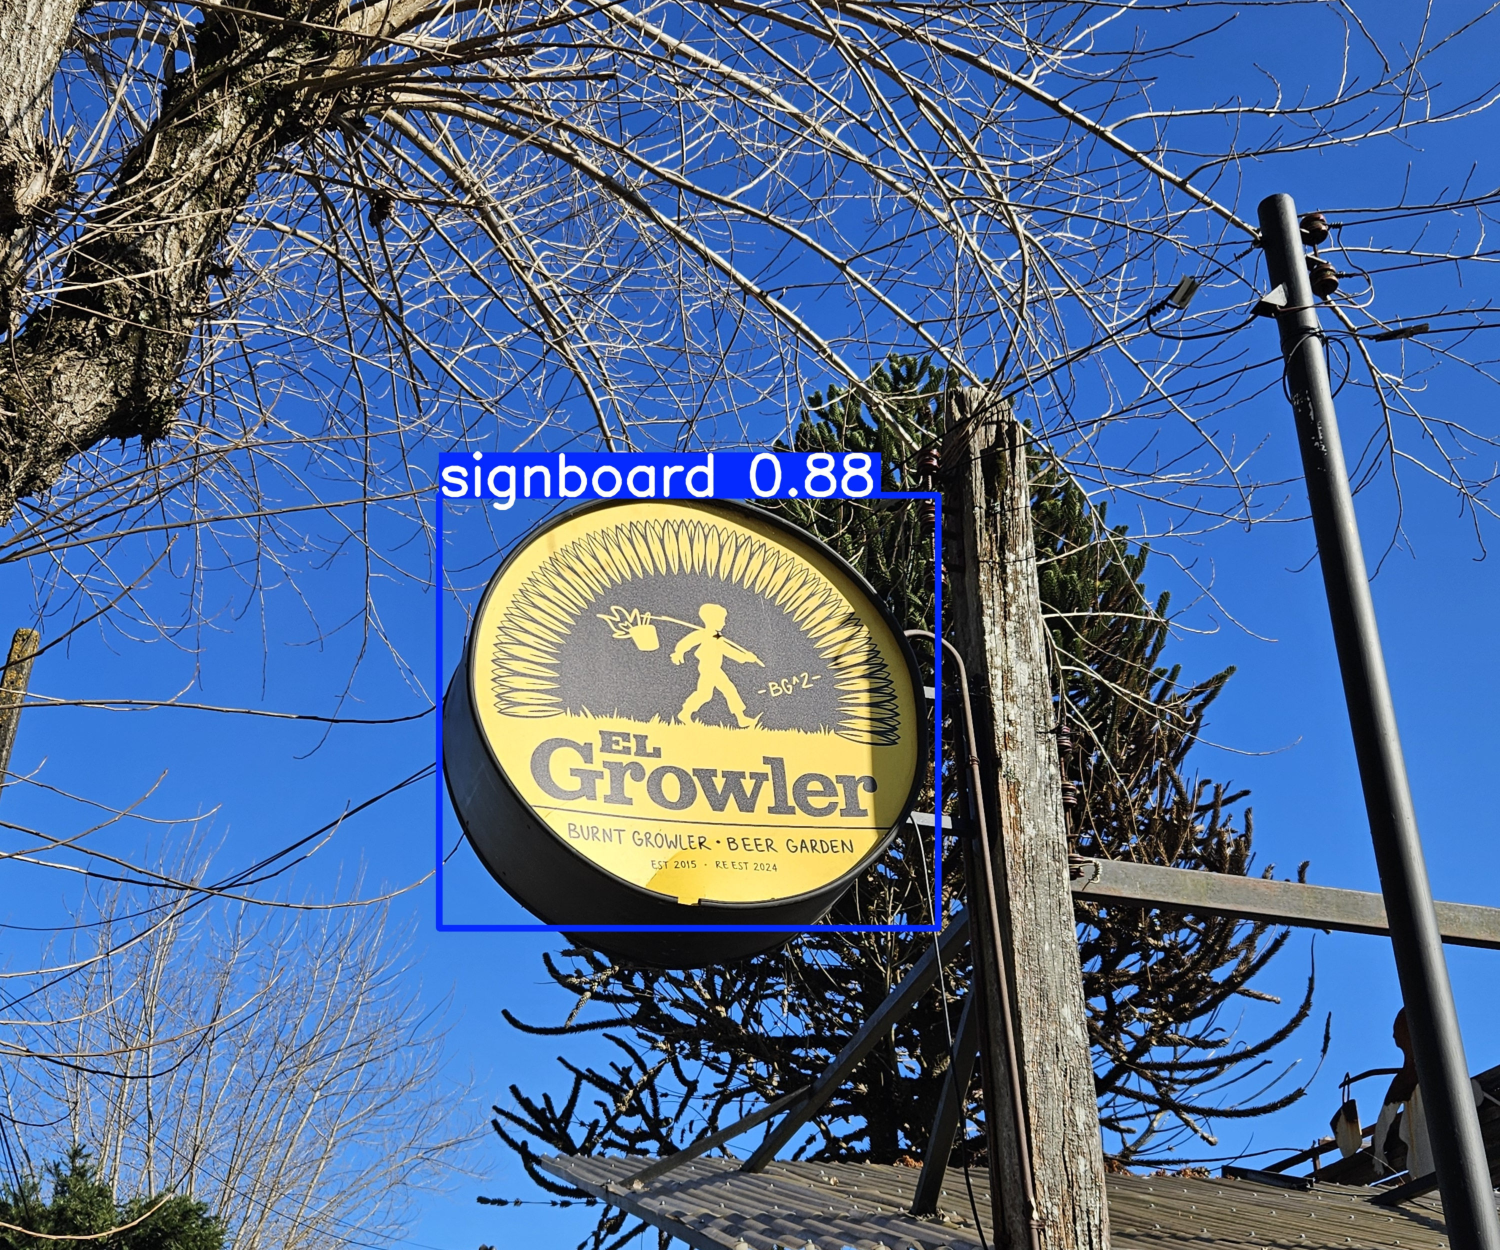
\includegraphics[width=\textwidth]{letreros_detectados/letrero1_comprimido.pdf}
    \end{subfigure}
    \hfill
    \begin{subfigure}[b]{0.23\textwidth}
        \centering
        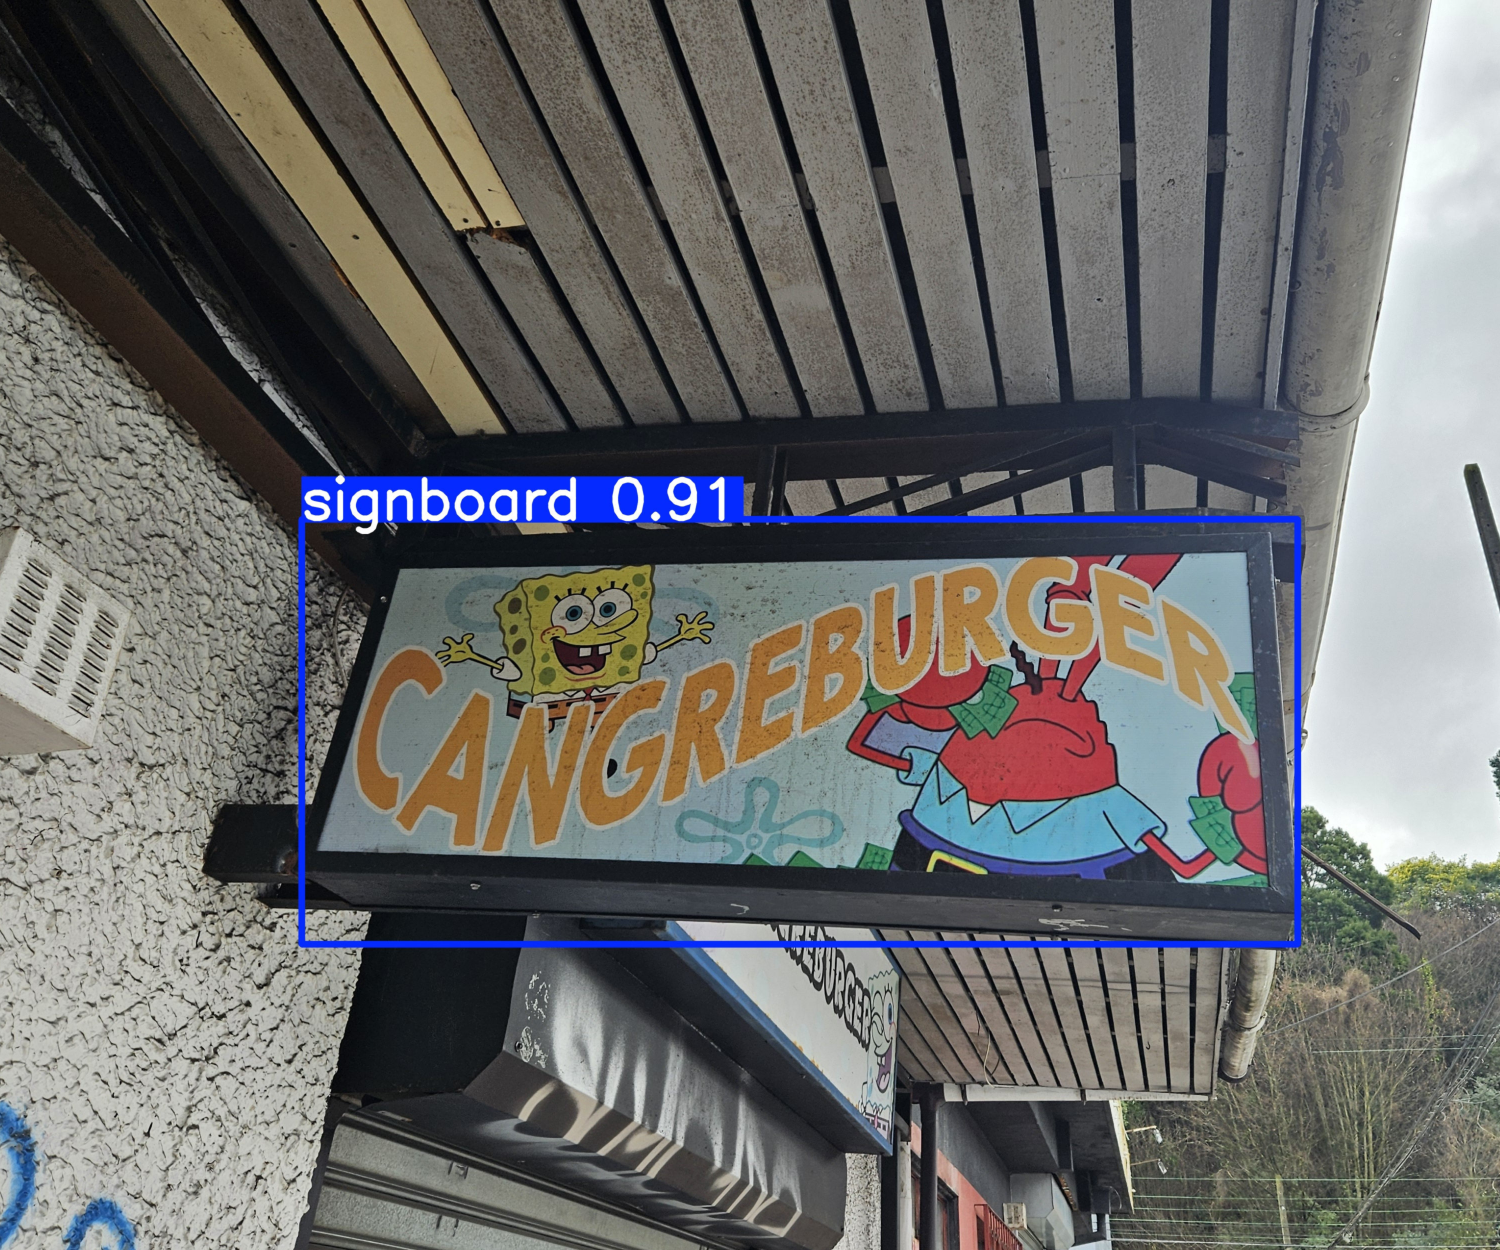
\includegraphics[width=\textwidth]{letreros_detectados/letrero4_comprimido.pdf}
    \end{subfigure}
    \hfill
    \begin{subfigure}[b]{0.23\textwidth}
        \centering
        
\includegraphics[width=\textwidth]{letreros_detectados/letrero3_comprimido.pdf}
    \end{subfigure}
    \hfill
    \begin{subfigure}[b]{0.23\textwidth}
        \centering
        
\includegraphics[width=\textwidth]{letreros_detectados/letrero2_comprimido.pdf}
    \end{subfigure}
    
    \caption{Detecciones del modelo YOLO11m-customizado sobre el conjunto de prueba.}
    \label{fig:letreros_rurales_detectados}
\end{figure}



\subsection{Etapa 2: Implementación del Modelo Detección de Letreros}
En esta subsección se describen los pasos necesarios para implementar 
el modelo de detección de letreros construido en la Etapa 1, siguiendo 
la secuencia definida en la Etapa 2 de la Figura~\ref{fig:pipeline}. 
El proceso abarca desde la captura de video y registro de 
geolocalización, la sincronización de ambas fuentes, la implementación 
del modelo de detección de letreros, la extracción de ROI (Region Of Interest) y procesamiento de 
imagen, el reconocimiento de texto mediante OCR, la identificación y 
categorización de las detecciones, hasta la visualización final de los 
resultados en un mapa interactivo.


\subsubsection{Captura de Video y Registro de Geolocalización}
\label{sec:captura}
Para la captura de datos en ruta se requiere un vehículo motorizado y 
un soporte para smartphone instalado en el tablero. El smartphone puede posicionarse de forma vertical u horizontal, siendo esta última la recomendada,
ya que proporciona mayor anchura en el 
encuadre y permite capturar mejor la señalética lateral de la ruta. 
Una vez el smartphone está en posición, se recomienda seguir un orden 
estricto de inicio y cierre: primero iniciar la grabación de 
geolocalización desde la aplicación GeoTracker (disponible para Android
e iOS) \cite{geotracker} y posteriormente iniciar la grabación de video desde la cámara nativa 
del smartphone. Este orden es relevante dado que, si se iniciara primero 
la grabación de video, los primeros frames capturados no tendrían una 
ubicación GPS asociada, lo que resultaría en la pérdida de letreros 
detectados en ese tramo. Al finalizar, se debe detener primero la 
grabación de video y luego la grabación de geolocalización, asegurando 
así que todos los frames del video cuenten con su correspondiente 
coordenada geográfica. Como resultado de este proceso se obtienen dos 
archivos: una grabación de video en formato \texttt{.mp4} y una traza 
de geolocalización en formato \texttt{.gpx}, ambos con marcas 
temporales que permiten su posterior sincronización.

\subsubsection{Implementación del Modelo de Detección de Letreros}
Con el video capturado se procede a 
aplicar el modelo de detección de letreros construido en la Etapa 1. El 
video de entrada es segmentado extrayendo un frame por segundo, siguiendo la 
misma frecuencia utilizada en la sincronización con la traza GPX. Cada 
frame extraído es enviado individualmente al modelo Yolo11m-customizado, 
el cual analiza la imagen y determina si contiene uno o más letreros. 
Para cada detección, el modelo retorna las coordenadas del bounding box y un score de confianza asociado,
reteniéndose únicamente aquellas cuya confianza supera el umbral de 0{,}5, valor establecido para aumentar la 
probabilidad de obtener detecciones correctas sin descartar letreros válidos capturados en condiciones adversas. 
Los frames con detecciones válidas, junto con sus coordenadas y scores, son 
almacenados para ser procesados en la etapa siguiente.

\subsubsection{Sincronización de Video y Geolocalizador}
La sincronización entre el video y la traza GPX es necesaria debido a 
que, en la práctica, ambas grabaciones no se inician en el mismo 
instante, generando inevitablemente un desfase temporal entre 
el inicio del video y el inicio del registro GPS. Para corregir este 
desfase, la sincronización se basa en alinear temporalmente ambas 
fuentes a partir de sus timestamps. Para ello, se extrae la metadata 
del video mediante la librería \texttt{pymediainfo} \cite{pymediainfo}, 
obteniendo la hora de creación del archivo y su duración en segundos. 
Dado que la hora de creación corresponde al instante en que el video 
fue finalizado, la hora de inicio se calcula como se define en la Ecuación~\ref{eq:sync}:

\begin{equation}
    t_{\text{inicio}} = t_{\text{fin}} - D
    \label{eq:sync}
\end{equation}

\noindent donde $t_{\text{fin}}$ corresponde a la hora de creación del 
archivo de video y $D$ a su duración en segundos. Ambos valores son 
convertidos a la zona horaria de Chile (\texttt{America/Santiago}) para 
garantizar consistencia con los timestamps del archivo GPX. Una vez 
establecido el intervalo temporal, la traza GPX es filtrada para 
extraer un registro por segundo, alineando cada punto GPS con el frame 
correspondiente y permitiendo que cada detección de letrero herede la 
coordenada geográfica de su instante exacto de captura.


\subsubsection{Extracción de ROI y Procesamiento de Imagen}
\label{sec:roi}
% bounding boxes, binarización (blanco y negro), limpieza, recortar deteccion, 

Una vez obtenidas las detecciones válidas del modelo, se procede a 
aislar la región de interés (ROI) correspondiente a cada letrero. A 
partir de las coordenadas del bounding box $(x_1, y_1, x_2, y_2)$ 
entregadas por el modelo, se recorta del frame original exclusivamente 
el área delimitada por dicho bounding box, descartando todo contenido 
circundante como vegetación, cielo o calzada. El resultado es una 
imagen reducida que contiene únicamente el letrero detectado.

Sobre esta ROI se aplica un proceso de \textit{thresholding} 
\cite{thresholding-para-mejorar-ocr}, técnica que consiste en convertir la imagen a 
escala de grises y binarizarla asignando a cada píxel el valor blanco 
o negro según su intensidad. Este proceso elimina variaciones de color 
y textura del fondo, generando una imagen de alto contraste que 
facilita significativamente la legibilidad del texto en la etapa de 
OCR posterior, especialmente en letreros con fondos de color, deterioro 
superficial o condiciones de iluminación no homogénea.

A continuación, en la Figura~\ref{fig:roi_ejemplo}, se presenta un 
ejemplo del proceso de extracción y preprocesamiento de una ROI, 
mostrando el recorte original del letrero detectado y su versión 
binarizada resultante del thresholding.

\begin{figure}[H]
    \centering
    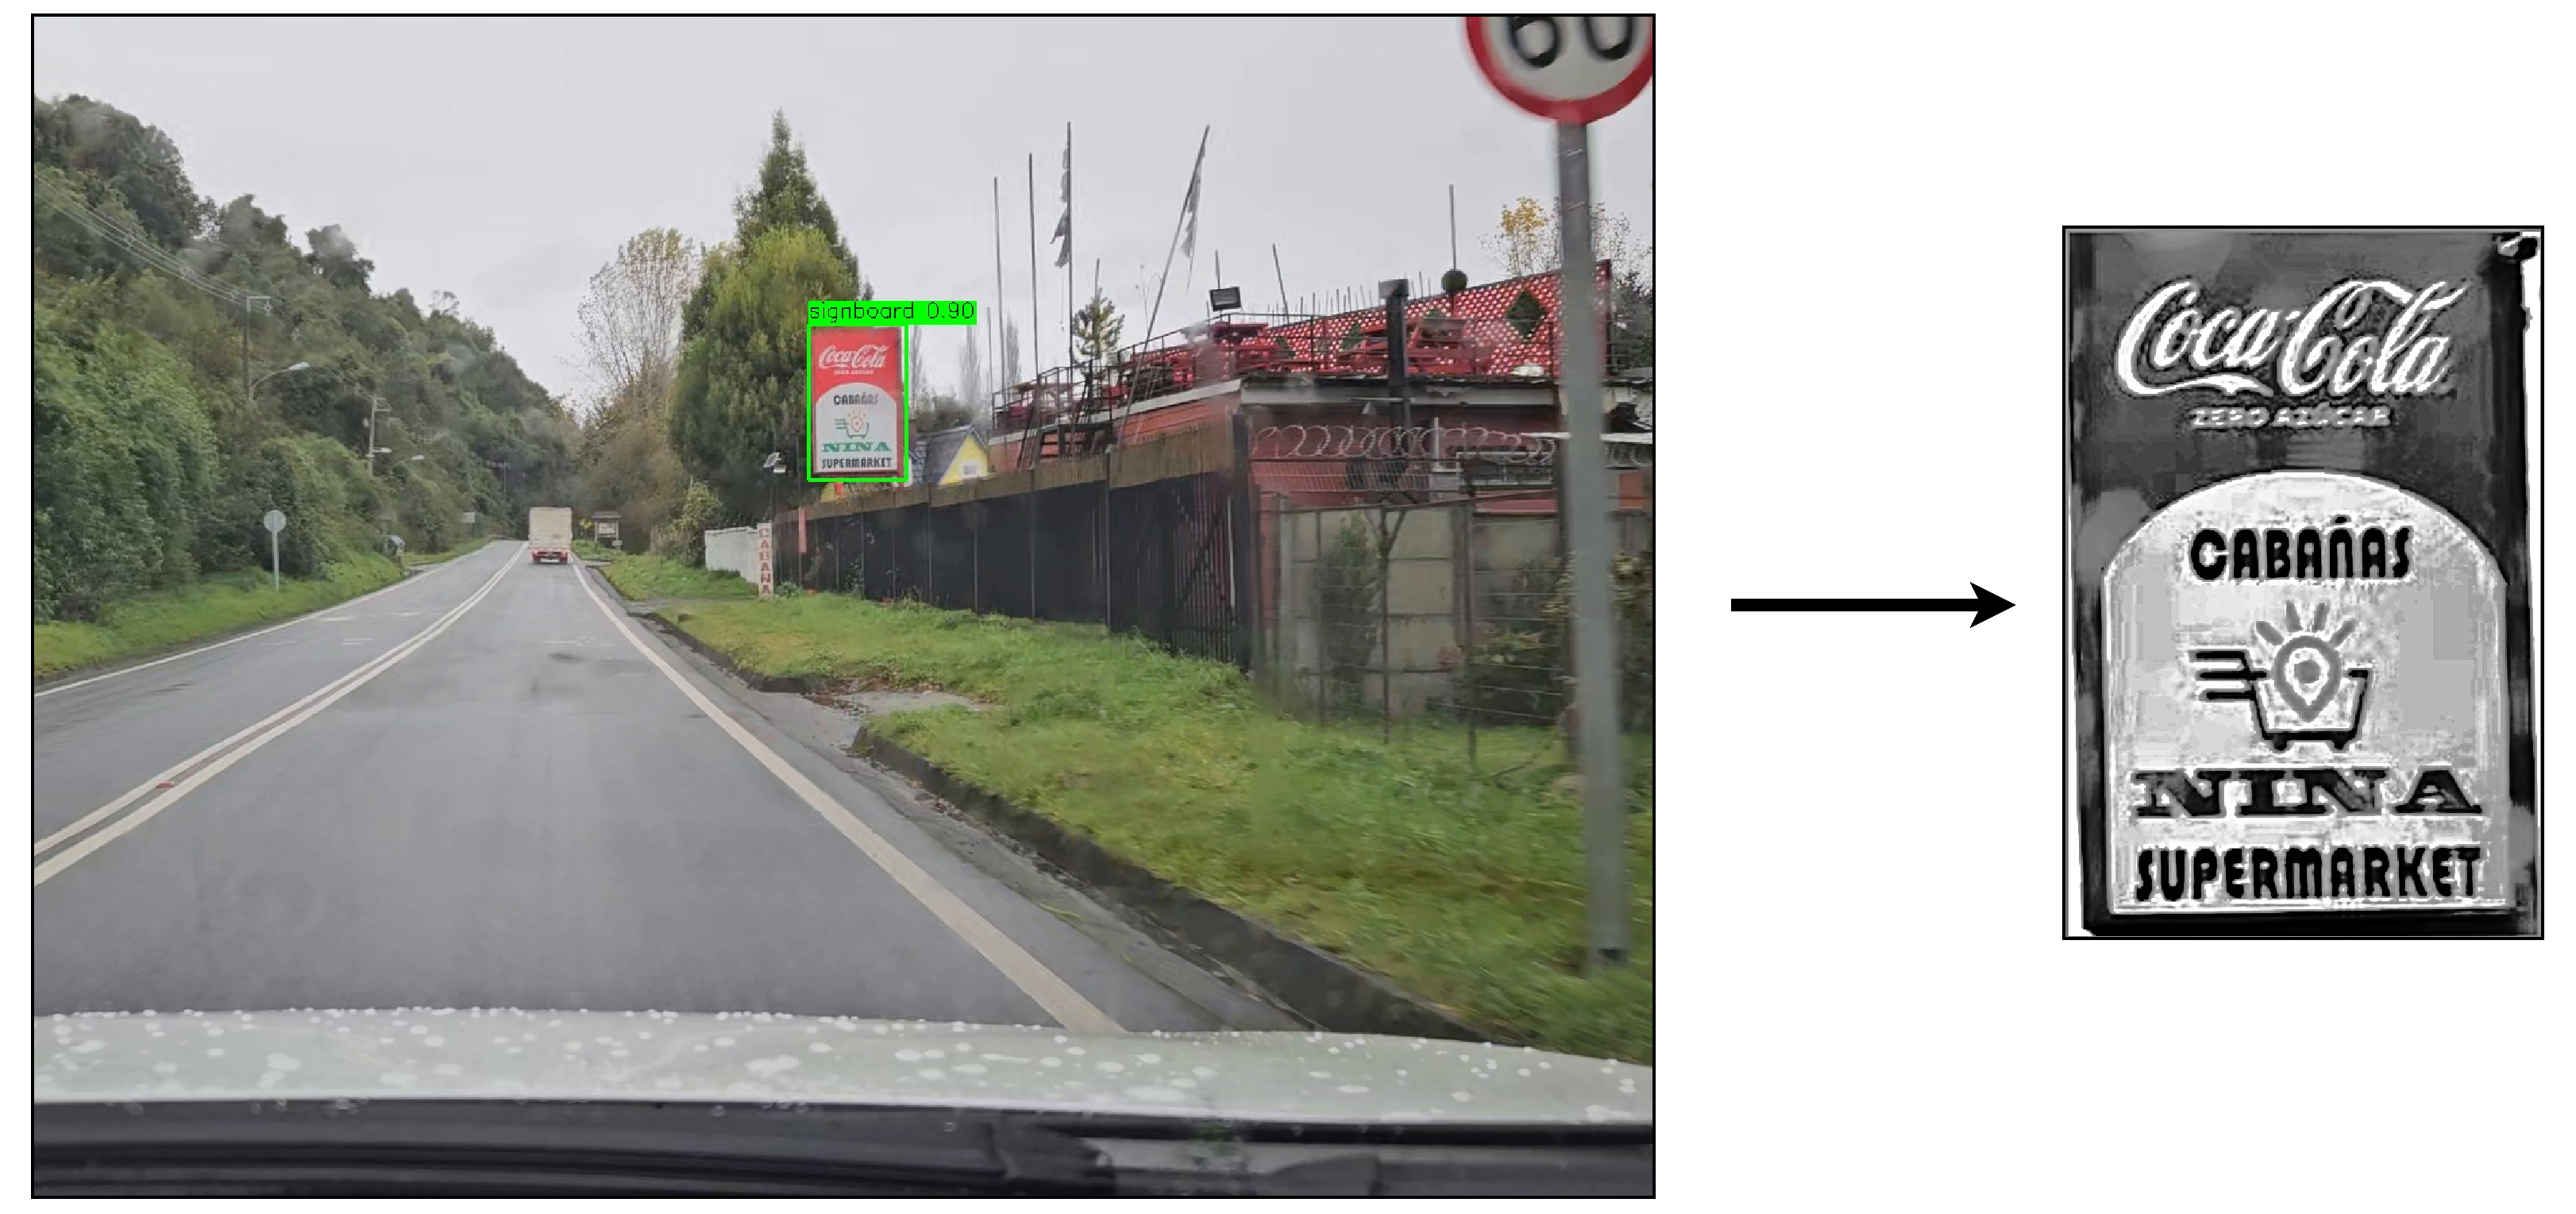
\includegraphics[width=0.5\linewidth]{letreros-roi/thresholing.pdf}
    \caption{Frame original con un letrero detectado (confianza: 0,9) a la izquierda y su versión binarizada mediante thresholding para el procesamiento OCR a la derecha.}
    \label{fig:roi_ejemplo}
\end{figure}

\subsubsection{Reconocimiento de Texto (OCR)}
\label{subsec:reconocimiento-ocr}
Para la extracción del contenido textual de cada ROI preprocesada se 
utilizó PaddleOCR \cite{paddleocr,paddleocr2}, una librería de código abierto 
desarrollada sobre el framework PaddlePaddle \cite{paddlepaddle} que ofrece soporte para múltiples idiomas, incluyendo español. PaddleOCR integra en un único 
pipeline tres etapas secuenciales: detección de las regiones de texto 
dentro de la imagen, ajuste geométrico de dichas regiones para 
corregir inclinaciones o perspectivas, y reconocimiento de los 
caracteres mediante una red neuronal de reconocimiento de secuencias. 
Cada ROI es procesada de forma individual y el algoritmo retorna, junto 
al texto reconocido, un valor de confianza (\textit{confidence}) entre 
0 y 1 que indica el nivel de certeza del modelo sobre el texto extraído. Con el fin de descartar reconocimientos 
poco confiables, se estableció un umbral mínimo de confianza de 0,5, 
determinado empíricamente mediante pruebas sobre un conjunto de videos 
de validación independientes de los utilizados en la experimentación 
final. Este filtro permite descartar casos como letreros con deterioro físico 
severo, frames afectados por motion blur que dificultan la 
legibilidad de los caracteres, y señalética de tránsito sin contenido 
alfanumérico detectada como producto del transfer learning, como señales 
de ceda el paso, señales de curva u otros indicadores viales con 
símbolos no textuales, cuyo contenido no es relevante para el dominio 
turístico. El texto reconocido que supera el umbral de confianza es 
almacenado junto con la detección correspondiente para su uso en las 
etapas posteriores de clasificación semántica por taxonomía y 
georreferenciación.

\subsubsection{Identificación y Categorización de las Detecciones}
Una vez extraído el texto de cada letrero mediante OCR, se procede a 
clasificar cada detección en una categoría semántica según su contenido. 
La taxonomía utilizada fue definida a partir de la clasificación de 
servicios turísticos propuesta por el gobierno de Chile 
\cite{taxonomia-gobierno}, adaptada al dominio específico de la 
señalética rural capturada en ruta, resultando en tres categorías 
principales: ``alojamiento'', ``alimentación'' y ``recreativa'', 
tal como se resume en la Tabla~\ref{tab:taxonomia}. Cualquier letrero 
cuyo texto no calce con ninguna de estas categorías es clasificado 
automáticamente como ``otros'', categoría que agrupa comúnmente 
señalética de venta de terrenos, talleres mecánicos y señalética 
de tránsito.

\begin{table}[H]
\centering
\caption{Taxonomía de clasificación semántica de letreros turísticos.}
\begin{tabular}{|c|c|c|}
\hline
\rowcolor{gray!20}
\textbf{Categoría} & \textbf{Cantidad de Palabras Clave} & \textbf{Ejemplos} \\
\hline
Alojamiento   & 17 & cabaña, hostal, hotel, hospedaje, apart hotel \\
\hline
Alimentación  & 73 & restaurant, picada, almuerzos, minimarket, comida casera \\
\hline
Recreativa    & 56 & rafting, cabalgatas, trekking, playa, artesanías \\
\hline
\end{tabular}
\label{tab:taxonomia}
\end{table}

La clasificación se implementó en Python mediante un diccionario de 
palabras clave asociadas a cada categoría. El texto extraído por el OCR 
es normalizado (eliminando tildes, mayúsculas y espacios) y comparado 
contra cada término de la taxonomía utilizando tanto coincidencia exacta 
como similitud difusa (\textit{fuzzy matching}) \cite{fuzzy-matching}, lo que permite 
identificar categorías incluso ante errores tipográficos o variaciones 
ortográficas propias del OCR. Un aspecto relevante de esta taxonomía es 
la incorporación de términos propios de la idiosincrasia y cultura 
chilena que no serían contemplados en clasificadores genéricos, tales 
como \textit{once}, \textit{fonda}, \textit{sopaipilla}, \textit{pan 
amasado}, \textit{mote con huesillo} y \textit{chochoca}, entre otros.

Adicionalmente, se implementó un algoritmo de evaluación de la calidad 
informativa de cada letrero detectado. Este algoritmo analiza el texto 
extraído mediante expresiones regulares en busca de elementos de 
contacto como números de teléfono, URLs o menciones de redes sociales, 
asignando uno de tres niveles: ``alto'' si el letrero contiene al menos 
un elemento de contacto; ``medio'' si fue correctamente clasificado en 
una categoría turística pero sin información de contacto; y ``bajo'' si 
la detección no aporta información relevante más allá del texto 
reconocido. Este esquema permite priorizar las detecciones según su 
utilidad para el usuario final.

\subsubsection{Visualización de Resultados}
% flujo completo, etapa de comunicacion del pipeline (video + grabacion-tracker), la salida de uno es la entrada del otro
Cada componente del pipeline es ejecutado de manera individual y manual, 
siguiendo el orden descrito en la Etapa 2 de la Figura~\ref{fig:pipeline}. Las salidas intermedias de cada etapa, tales como imágenes de frames, 
ROIs procesadas y detecciones, son almacenadas en carpetas organizadas 
por video, mientras que la información estructurada generada en cada 
paso es guardada en archivos CSV independientes. Una vez completadas todas las etapas, se realiza una consolidación final mediante un script en Python que utiliza 
la librería \texttt{Pandas} \cite{pandas} para combinar y manipular todos los CSV generados, 
produciendo un archivo Excel con el registro completo de todas 
las detecciones georreferenciadas. Este archivo es integrado en un 
Sistema de Información Geográfica (SIG) \cite{sig-referencia}, donde 
cada detección es representada como un punto georreferenciado en un 
mapa interactivo, presentando la ubicación de cada letrero junto con 
la información extraída a lo largo de las rutas recorridas.

% =====================================================
\section{Configuración Experimental}
En esta sección se describen las condiciones bajo las cuales fue 
evaluado el pipeline GEODETECTOR, incluyendo el entorno de hardware 
y software utilizado, las métricas de evaluación y los escenarios
experimentales.

\subsection{Hardware y Software}
% GPU, CPU

El pipeline fue ejecutado íntegramente en el supercomputador Patagón 
de la Universidad Austral de Chile (UACh) \cite{patagon}, accediendo 
a sus recursos de forma remota mediante conexión SSH (Secure Shell) desde Visual 
Studio Code \cite{vscode}, que actuó como entorno de desarrollo e interfaz principal 
de trabajo. Para las etapas de mayor demanda computacional 
(entrenamiento del modelo, inferencia de detección y procesamiento 
OCR) se empleó una GPU NVIDIA L40, cuyas características de memoria 
y capacidad de cómputo paralelo resultan adecuadas para operaciones 
intensivas sobre redes neuronales profundas. Para el resto de los 
programas con menor exigencia computacional, como la sincronización de 
coordenadas GPS con el video y la consolidación de resultados, se 
empleó una GPU NVIDIA RTX A4000.

En cuanto al software, el pipeline fue desarrollado íntegramente en 
Python \cite{python2026}, utilizando las siguientes librerías 
principales: \texttt{Ultralytics} para el entrenamiento e inferencia con 
YOLO11 \cite{yolo11_ultralytics}, \texttt{PaddleOCR} para el reconocimiento 
de texto \cite{paddleocr}, \texttt{OpenCV} \cite{opencv} para el procesamiento de imagen, y \texttt{Pandas} \cite{pandas} para la manipulación y 
consolidación de los datos generados. Adicionalmente, se utilizaron 
otras librerías complementarias descritas en las secciones anteriores, 
las cuales fueron igualmente ejecutadas en el entorno del 
supercomputador Patagón.


\subsection{Métricas de Evaluación}
%  precision, recall, pero respecto a la deteccion y de conteo manual (esta metrica tiene que ver con el modelo), mla matriz de confunsion
% manual muestra esto
% Calidad del texto detectado (de todos los letreros detectados y ocr, cuantos dice exactamente lo mismo que el frame real). Nivel de similitud del texto
% vamos a medir la similitud del texto original vs el texto detectado con OCR)
% vamos a medir de los textos detectados 
Para evaluar el desempeño del pipeline se consideraron dos dimensiones:
 la calidad de la detección de letreros y la calidad del reconocimiento
  de texto mediante OCR.

\subsubsection{Evaluación de la Detección de Letreros}
\label{subsec:evaluacion-deteccion}

La detección de letreros se evaluó mediante las métricas de \textit{Precisión}, \textit{Recall} y \textit{F1-score}, ampliamente utilizadas en tareas de detección de objetos, tal como se presenta en la Ecuación~\ref{eq:metricas}.
La Precisión mide la proporción de detecciones correctas sobre el total de detecciones realizadas, mientras que el Recall mide la proporción de letreros reales
que fueron efectivamente detectados. Por su parte, el F1-score corresponde a la media armónica entre Precisión y Recall, permitiendo evaluar el equilibrio entre ambas métricas.
Para obtener el \textit{ground truth} (verdad fundamental) \cite{ibm_ground_truth}, se realizó un conteo manual frame por frame a razón de un frame por segundo, identificando los 
letreros presentes en cada instante de los tres videos de prueba, capturados bajo distintas condiciones de iluminación y clima.

Formalmente:

\begin{equation}
\text{Precisión} = \frac{TP}{TP + FP}, \quad
\text{Recall} = \frac{TP}{TP + FN}, \quad
F1 = 2 \cdot \frac{\text{Precisión} \cdot \text{Recall}}{\text{Precisión} + \text{Recall}}
\label{eq:metricas}
\end{equation}

donde TP corresponde a los letreros correctamente detectados por el 
modelo (verdaderos positivos), FP a las detecciones incorrectas 
realizadas por el modelo (falsos positivos) y FN a los letreros presentes
 en la escena que no fueron detectados (falsos negativos).

\subsubsection{Evaluación del OCR}
\label{subsec:evaluacion-ocr}
Para medir la calidad del texto reconocido, se comparó el texto extraído 
por el módulo OCR contra el texto real de cada letrero, obtenido mediante 
transcripción manual de los letreros detectados en el ground truth. La métrica
utilizada es el \textit{Character Error Rate} (CER), o Tasa de Error de Caracteres \cite{schaefer2020ocr}, estándar en la literatura de OCR, que 
mide la proporción de caracteres incorrectos entre el texto reconocido 
y el texto real, tal como se muestra en la Ecuación~\ref{eq:cer}:

\begin{equation}
CER = \frac{S + D + I}{N}
\label{eq:cer}
\end{equation}

donde $S$ corresponde a sustituciones, $D$ a eliminaciones, $I$ a 
inserciones de caracteres y $N$ al total de caracteres del texto real. 
Los valores de $S$, $D$ e $I$ se obtienen mediante el algoritmo de 
distancia de edición de Levenshtein \cite{levenshtein1966binary}, que 
determina la secuencia mínima de operaciones necesarias para transformar 
el texto reconocido en el texto real, implementado en Python sobre cada 
par de textos evaluados. Para la interpretación de los resultados se 
definen rangos de referencia adaptados del estándar utilizado en 
plataformas de reconocimiento de texto \cite{transkribus-cer}, ajustados 
al dominio de escenas naturales donde los valores de CER son 
inherentemente mayores que en documentos estructurados, tal como se 
presenta en la Tabla~\ref{tab:rangos_cer}. Para cada escenario 
evaluado se reporta el CER promedio calculado sobre el conjunto de 
letreros detectados, filtrados y clasificados en dicha configuración.

\begin{table}[H]
\centering
\caption{Interpretación de los valores de CER utilizados como referencia.}
\label{tab:rangos_cer}
\begin{tabular}{|c|c|>{\centering\arraybackslash}p{8cm}|}
\hline
\rowcolor{gray!20}
\textbf{Rango de CER} & \textbf{Interpretación} & \textbf{Descripción} \\
\hline
$CER = 0$ & Perfecto (P) & Reconocimiento perfecto, sin errores de OCR. \\
\hline
$0 < CER \leq 0.05$ & Excelente (E) & Desempeño excelente, con muy pocos errores de reconocimiento. \\
\hline
$0.05 < CER \leq 0.10$ & Bueno (B) & Desempeño bueno y suficiente para la mayoría de aplicaciones prácticas. \\
\hline
$0.10 < CER \leq 0.20$ & Aceptable (A) & Desempeño aceptable, aunque con errores perceptibles en el texto reconocido. \\
\hline
$CER > 0.20$ & Deficiente (D) & Desempeño deficiente, con una alta cantidad de errores de OCR. \\
\hline
\end{tabular}
\end{table}


\subsection{Escenarios Experimentales}
% día, noche, clima, velocidad
% se van a medir a medir distintos escenarios experimentales, con 4 videos que presentan condiciones y configuraciones de captura
% de video, las evaluaciones son: 2 videos dia, 2 noche, 2 tarde. Estos videos varian entre 50-80 km/h
% tabla 
Los tres videos base fueron capturados con un smartphone Samsung Galaxy 
S23 en formato \texttt{.mp4} y en su resolución nativa de 1080p a 30 FPS, 
bajo condiciones variables de iluminación y clima, a velocidades de 
entre 50 y 70 km/h. Con el fin de evaluar el impacto de la calidad de 
captura sobre el desempeño del pipeline, cada video original fue 
procesado mediante el framework \texttt{FFmpeg} \cite{ffmpeg} para generar tres 
variantes adicionales: 1080p a 15 FPS, 720p a 30 FPS y 720p a 15 FPS. 
De esta forma, cada video base da origen a cuatro configuraciones 
distintas, resultando en un total de 12 escenarios experimentales sobre 
los mismos videos. En la Tabla~\ref{tab:escenarios} resume las condiciones
 de captura en ruta y experimentación de cada video base, donde \textbf{LR}
  corresponde a la cantidad total de Letreros Reales observados en la
   escena, independientemente de su categoría o de si forman parte de 
   la taxonomía considerada en este trabajo, y \textbf{LRT} a la cantidad 
   de Letreros Reales Turísticos, estos últimos definidos según la 
   taxonomía presentada en la Tabla~\ref{tab:taxonomia}. Ambas cantidades
    fueron obtenidas mediante conteo manual.

\begin{table}[H]
\centering
\caption{Escenarios experimentales evaluados.}
\begin{tabular}{|c|c|c|c|c|c|c|c|c|c|c|}
\hline
\rowcolor{gray!20}
\textbf{Video} & \textbf{Sector} & \textbf{Hora} & \textbf{Duración} & \textbf{Periodo} & \textbf{Clima} & \textbf{Velocidad} & \textbf{LR} & \textbf{LRT} & \textbf{Resolución} & \textbf{FPS} \\
\hline
V1 & Carretera Austral & 11:13 & 4:03 min & Mañana & Lluvia    & 50--70 km/h & 87 & 23 & 1080p/720p & 30/15 \\
\hline
V2 & Río Maullín & 10:17 & 4:13 min & Mañana & Neblina   & 50--70 km/h & 34 & 4 & 1080p/720p & 30/15 \\
\hline
V3 & Camino a Ensenada & 16:52 & 5:58 min & Tarde  & Despejado & 50--70 km/h & 91 & 19 & 1080p/720p & 30/15 \\
\hline
\end{tabular}
\label{tab:escenarios}
\end{table}


% =====================================================
\section{Resultados Experimentales}
% aqui vamos a definir el ground truht son 4 videos de 3 minutos (la tabla de wsl)
% los escenarios experimentales condiciones... 
% en la presente tabla de presenta los resultados reales. agregar otra columna con la duracion del video
% esta tabla esta en wsp, define los videos 
En esta sección se presentan los resultados obtenidos al ejecutar el 
pipeline GEODETECTOR sobre los tres videos de prueba en sus distintas 
configuraciones de resolución y FPS. Los resultados se organizan en cuatro 
dimensiones: resultados de detección de letreros, resultados de OCR, evaluación end-to-end
y resultados cualitativos.


% esto va dps de la tabla: cada uno de los 4 videos poaso por un proceso de transformación de FPS (15/30) y resolución (720/480),
%dando un total de 16 escenarios esperimentales, es decir, (Vx, 15, 720), (Vx, 30, 720) (Vx, 15, 480), (Vx, 30, 480). 
%Bajos este conjunto de escenarios validaremos ground truth.
% Adicionalmente, se evaluará el pipeline completo con 2 videos, uno de 15 minutos y unos de 17 min.

% video 1, tiene velocidad de 1 minuto de [50-60], en el minuto 2 de [60-70] hasta el minuto 3 donde termina

\subsection{Resultados de Detección de Letreros}
% ground truth: métricas modelo. contar a mano los letreros y ver cuantos detectó el modelo. aqui va la matriz de confunsion a mano
% Esta es la tabla .. para validar la calidad del modelo. ademas esta tabla (ver foto de wsp)
% cada uno de los 4 videos poaso por un proceso de transformación de FPS (15/30) y resolución (720/480), dando un total de 16 escenarios esperimentales, es decir, (Vx, 15, 720), (Vx, 30, 720) (Vx, 15, 480), (Vx, 30, 480). Bajos este conjunto de escenarios validaremos ground truth.
% Adicionalmente, se evaluará el pipeline completo con 2 videos, uno de 15 minutos y unos de 17 min.
\label{subsec:resultados-deteccion}

En la Tabla~\ref{tab:deteccion} presenta los resultados de detección de 
letreros para cada video y configuración, utilizando como ground truth
 (verdad fundamental) un conteo manual efectuado sobre los frames con
  detecciones generados por el modelo. Dicho conteo permitió determinar
   los valores de verdaderos positivos (TP), falsos positivos (FP) y 
   falsos negativos (FN). Adicionalmente, se evaluaron manualmente los
    LRT definidos en la Tabla~\ref{tab:escenarios} respecto de los
TP obtenidos por el modelo, dando como resultado la columna \textbf{LRT-TP},
que indica, en notación \textit{cantidad/total}, cuántos letreros 
turísticos reales (LRT) fueron correctamente detectados (TP) respecto 
al total de letreros turísticos presentes en cada video según el 
ground truth.


\begin{table}[H]
\centering
\caption{Resultados de detección de letreros por video y configuración.}
\begin{tabular}{|c|c|c|c|c|c|c|c|c|c|}
\hline
\rowcolor{gray!20}
\textbf{Video} & \textbf{Resolución} & \textbf{FPS} & \textbf{TP} & \textbf{FP} & \textbf{FN} & \textbf{Precisión} & \textbf{Recall} & \textbf{F1-Score} & \textbf{LRT-TP} \\
\hline
V1 & 1080p & 30 & 55 & 8 & 32 & 0,87 & 0,63 & 0,73 & 21/23\\
\hline
V1 & 1080p & 15 & 52 & 9 & 35 & 0,85 & 0,60 & 0,70 & 20/23\\
\hline
V1 & 720p  & 30 & 52 & 5 & 35 & 0,91 & 0,60 & 0,72 & 21/23\\
\hline
V1 & 720p  & 15 & 45 & 6 & 42 & 0,88 & 0,52 & 0,65 & 20/23\\
\hline
V2 & 1080p & 30 & 21 & 4 & 13 & 0,84 & 0,62 & 0,71 & 3/4\\
\hline
V2 & 1080p & 15 & 25 & 7 & 9 & 0,78 & 0,74 & 0,76 & 3/4\\
\hline
V2 & 720p  & 30 & 18 & 3 & 16 & 0,86 & 0,53 & 0,66 & 3/4\\
\hline
V2 & 720p  & 15 & 17 & 5 & 17 & 0,77 & 0,50 & 0,61 & 3/4\\
\hline
V3 & 1080p & 30 & 57 & 10 & 34 & 0,85 & 0,63 & 0,72 & 18/19\\
\hline
V3 & 1080p & 15 & 61 & 13 & 30 & 0,81 & 0,67 & 0,73 & 17/19\\
\hline
V3 & 720p  & 30 & 50 & 11 & 41 & 0,82 & 0,55 & 0,66 & 16/19\\
\hline
V3 & 720p  & 15 & 54 & 7 & 37 & 0,89 & 0,59 & 0,72 & 15/19\\
\hline
\end{tabular}
\label{tab:deteccion}
\end{table}


Los resultados de detección de letreros se obtuvieron aplicando las 
métricas definidas en la Subsección~\ref{subsec:evaluacion-deteccion}, 
donde a partir de los valores de TP, FP y FN se calculan la Precisión, 
Recall y F1-Score según la Ecuación~\ref{eq:metricas}. En términos generales, la Precisión se mantiene 
relativamente estable entre configuraciones, oscilando entre $0,77$ y 
$0,91$, lo que indica que el modelo es consistente en evitar falsos 
positivos independientemente de la calidad del video. El Recall, en 
cambio, muestra mayor sensibilidad a la reducción de FPS, oscilando 
entre $0,50$ y $0,74$, sugiriendo que una menor tasa de frames aumenta 
la probabilidad de no detectar letreros que aparecen brevemente en 
escena. Respecto al F1-Score, los valores oscilan entre $0,61$ y 
$0,76$, reflejando el equilibrio entre precisión y exhaustividad. 
V2 (neblina) obtiene los menores valores absolutos de TP, 
comportamiento atribuible tanto a las condiciones climáticas adversas 
como a la menor densidad de letreros en su recorrido (34 letreros 
reales). V3 (despejado) presenta el mayor F1-Score promedio entre los 
tres videos, confirmando que las condiciones de iluminación favorables 
impactan positivamente el desempeño del modelo. Respecto a la columna 
\textbf{LRT-TP}, V1 concentra la mayor densidad de señalética turística con 
20 a 21 detecciones relevantes por configuración, mientras que V2 
presenta solo 3, diferencia que no solo refleja el impacto de las 
condiciones climáticas, sino también la menor oferta turística presente 
en la zona geográfica recorrida por dicho video, en comparación con 
las rutas de V1 y V3.


\subsection{Resultados de OCR}
\label{subsec:resultados-ocr}

A partir de los \textbf{LRT-TP} presentados en la 
Tabla~\ref{tab:deteccion}, la Tabla~\ref{tab:ocr} incorpora dos 
columnas adicionales en la misma notación \textit{cantidad/total} 
para dar seguimiento al flujo de información a través del módulo OCR. 
Tanto \textbf{LRT-TP} como \textbf{LE-LRT} forman parte del ground 
truth, en tanto su segundo valor representa la cantidad real de 
letreros turísticos presentes en el video, obtenida mediante conteo 
manual. La columna \textbf{LE-LRT} (Letreros Evaluados de 
Letreros Reales Turísticos) se expresa como $x/LRT$, donde $x$ 
corresponde a la cantidad de letreros turísticos reales correctamente 
detectados que además superaron el umbral de confianza OCR y fueron 
evaluados con la métrica CER, y $LRT$ corresponde al total de letreros 
turísticos reales presentes en el video según el ground truth. Por su 
parte, la columna \textbf{LE-CER} (Letreros Evaluados con la métrica 
CER) se expresa como $x/(TP+FP)$, donde $x$ corresponde a la cantidad 
de letreros que superaron el umbral mínimo de confianza OCR 
y fueron evaluados mediante la métrica CER, mientras que $TP+FP$ 
representa el total de detecciones realizadas por el modelo en dicha 
configuración, incluyendo tanto detecciones correctas como incorrectas. 
Los letreros descartados, tanto turísticos como de otras categorías, se 
atribuyen principalmente a señalética con deterioro físico, 
letreros de tránsito sin contenido alfanumérico como señales de curva 
o advertencia, y frames con borrosidad producto del desenfoque por 
movimiento (\textit{motion blur}), cuya nitidez insuficiente impide al 
módulo OCR reconocer el texto con una confianza igual o superior a 
establecida. Para cada letrero evaluado, el texto extraído por el módulo OCR 
fue comparado contra el texto real obtenido mediante transcripción 
manual del frame correspondiente. Además, se presenta los resultados expresados como el 
CER promedio (\textbf{CER prom.}) de cada configuración, calculado 
promediando el CER individual obtenido para cada letrero evaluado, 
según la Ecuación~\ref{eq:cer}. Adicionalmente, las columnas \textbf{P},
\textbf{E}, \textbf{B}, 
\textbf{A} y \textbf{D} indican la cantidad de letreros cuyo CER 
individual cayó en cada uno de los rangos definidos en la 
Tabla~\ref{tab:rangos_cer}: Perfecto (P), Excelente (E), Bueno (B), 
Aceptable (A) y Deficiente (D). Por su parte, la columna 
\textbf{Interpretación prom.} corresponde al nivel de interpretación 
asociado al valor de CER promedio de la configuración, según los 
mismos rangos de dicha tabla.


\begin{table}[H]
\centering
\caption{Resultados de OCR por video y configuración.}
\begin{tabular}{|c|c|c|c|c|c|c|c|c|c|c|c|c|}
\hline
\rowcolor{gray!20}
\textbf{Video} & \textbf{Resolución} & \textbf{FPS} & \textbf{LRT-TP} & \textbf{LE-LRT} & \textbf{LE-CER} & \textbf{P} & \textbf{E} & \textbf{B} & \textbf{A} & \textbf{D} & \textbf{CER prom.} & \textbf{Interpretación prom.} \\
\hline
V1 & 1080p & 30 & 21/23 & 11/23 & 22/63 & 8 & 3 & 3 & 3 & 5 & 0,13 & Aceptable \\
\hline
V1 & 1080p & 15 & 20/23 & 8/23 & 19/61 & 4 & 1 & 2 & 4 & 8 & 0,23 & Deficiente \\
\hline
V1 & 720p  & 30 & 21/23 & 6/23 & 14/57 & 4 & 1 & 2 & 3 & 4 & 0,16 & Aceptable \\
\hline
V1 & 720p  & 15 & 20/23 & 7/23 & 15/51 & 3 & 3 & 3 & 0 & 6 & 0,22 & Deficiente \\
\hline
V2 & 1080p & 30 & 3/4 & 3/4 & 15/25 & 9 & 0 & 2 & 3 & 1 & 0,08 & Bueno \\
\hline
V2 & 1080p & 15 & 3/4 & 2/4 & 12/32 & 2 & 2 & 1 & 2 & 5 & 0,27 & Deficiente \\
\hline
V2 & 720p  & 30 & 3/4 & 1/4 & 9/21 & 2 & 1 & 1 & 2 & 3 & 0,16 & Aceptable \\
\hline
V2 & 720p  & 15 & 3/4 & 0/4 & 8/22 & 1 & 0 & 3 & 1 & 3 & 0,16 & Aceptable \\
\hline
V3 & 1080p & 30 & 18/19 & 10/19 & 35/67 & 14 & 6 & 5 & 5 & 5 & 0,10 & Bueno \\
\hline
V3 & 1080p & 15 & 17/19 & 8/19 & 27/74 & 7 & 2 & 7 & 3 & 8 & 0,20 & Aceptable \\
\hline
V3 & 720p  & 30 & 16/19 & 7/19 & 24/61 & 5 & 0 & 1 & 7 & 11 & 0,24 & Deficiente \\
\hline
V3 & 720p  & 15 & 15/19 & 6/19 & 24/61 & 6 & 1 & 5 & 4 & 8 & 0,21 & Deficiente \\
\hline
\end{tabular}
\label{tab:ocr}
\end{table}

Los resultados revelan un comportamiento 
heterogéneo del módulo OCR según las condiciones de captura. En V1 
(lluvia), las configuraciones de 30 FPS obtienen CER aceptables 
(0,13 en 1080p y 0,16 en 720p), mientras que la reducción a 15 FPS 
eleva el error a niveles deficientes (0,23 y 0,22 respectivamente), 
sugiriendo que la tasa de frames es un factor crítico bajo condiciones 
climáticas adversas. V2 (neblina) presenta el mejor resultado en 
1080p a 30 FPS con un CER de 0,08 (bueno), aunque con solo 15 letreros 
evaluados, lo que limita la representatividad de ese resultado. Sin 
embargo, la reducción a 15 FPS en V2 produce la mayor caída observada 
en toda la tabla, pasando a un CER de 0,27 (deficiente). V3 
(despejado) muestra el comportamiento más estable: 1080p a 30 FPS 
alcanza un CER de 0,10 (bueno) con 35 letreros evaluados, siendo la 
configuración con mayor cantidad de letreros y mejor representatividad. 
En general, la configuración de 1080p a 30 FPS es la que obtiene 
consistentemente los mejores resultados en todos los videos, mientras 
que las configuraciones de 15 FPS tienden a degradar significativamente 
el desempeño del OCR independientemente de la resolución, lo que 
sugiere que la tasa de frames tiene mayor impacto sobre el 
reconocimiento de texto que la resolución por sí sola.

\subsection{Evaluación End-to-End}
% sistema completo
La evaluación integral del pipeline considera el desempeño conjunto 
de todas sus etapas, desde la captura del video y la sincronización 
GPS hasta la visualización georreferenciada del letrero clasificado. 
A diferencia de las métricas individuales de detección de letreros y OCR 
presentadas anteriormente, esta evaluación considera el resultado 
final que el pipeline entrega de forma automática al usuario: un 
letrero correctamente detectado, con su texto reconocido, clasificado 
en una categoría turística, con su calidad de contenido identificada 
y categorizada, y posicionado en el mapa con sus coordenadas reales. 
Los resultados experimentales demuestran que el pipeline logra 
completar este flujo de forma exitosa en los escenarios de mayor 
calidad de captura (1080p, 30 FPS), con una degradación progresiva a 
medida que disminuye la resolución y la tasa de frames, consistente 
con los resultados individuales reportados en las 
Subsecciones~\ref{subsec:resultados-deteccion} 
y~\ref{subsec:resultados-ocr}. Cabe destacar que la identificación de 
cuáles detecciones corresponden efectivamente a letreros turísticos 
reales (LRT) constituye una verificación manual realizada con fines 
de evaluación, mientras que el pipeline en sí opera de forma 
automática sobre la totalidad de las detecciones, sin distinguir a 
priori entre categorías turísticas y no turísticas.

Considerando la configuración original (1080p, 30 FPS) de los tres 
videos, el flujo completo del pipeline se describe a continuación. 
En V1 (Carretera Austral), de los 87 (LR) letreros reales presentes en la 
ruta, el modelo detectó automáticamente 55 (TP), generó 8 falsas 
detecciones (FP) y no detectó 32 (FN), totalizando 63 detecciones 
(TP+FP) enviadas al módulo OCR. De los 23 letreros turísticos reales 
(LRT) presentes en la ruta, la verificación manual identificó que 21 
de ellos fueron correctamente detectados (LRT-TP), incluidos dentro 
de los 55 TP totales. De las 63 detecciones procesadas por el OCR, 
solo 22 superaron el umbral de confianza de $0,5$ (LE-CER), siendo 
descartadas las 41 restantes por razones como deterioro físico, 
señalética de tránsito sin contenido alfanumérico, falsas detecciones 
o borrosidad producto del \textit{motion blur}. De estos 22 letreros 
evaluados con CER, la verificación manual determinó que 11 
correspondieron efectivamente a letreros turísticos (LE-LRT) y los 11 
restantes a otras categorías fuera de la taxonomía turística definida 
en la Tabla~\ref{tab:taxonomia}. Esto indica que, de los 21 letreros 
turísticos correctamente detectados por el modelo, solo 11 lograron 
superar el umbral de confianza OCR y ser efectivamente evaluados y 
clasificados por el pipeline.

En V2 (Río Maullín), de los 34 (LR) letreros reales presentes en la ruta, 
el modelo detectó automáticamente 21 (TP), generó 4 falsas 
detecciones (FP) y no detectó 13 (FN), totalizando 25 detecciones 
enviadas al OCR. De los 4 letreros turísticos reales presentes, la 
verificación manual identificó 3 correctamente detectados (LRT-TP). 
De las 25 detecciones procesadas, 15 superaron el umbral de confianza 
(LE-CER), de las cuales 3 correspondieron efectivamente a letreros 
turísticos (LE-LRT), es decir, la totalidad de los letreros 
turísticos detectados por el modelo en este video logró ser evaluada 
y clasificada por el pipeline.

En V3 (Camino a Ensenada), de los 91 (LR) letreros reales presentes en la 
ruta, el modelo detectó automáticamente 57 (TP), generó 10 falsas 
detecciones (FP) y no detectó 34 (FN), totalizando 67 detecciones 
enviadas al OCR. De los 19 letreros turísticos reales presentes, la 
verificación manual identificó 18 correctamente detectados (LRT-TP). 
De las 67 detecciones procesadas, 35 superaron el umbral de confianza 
(LE-CER), de las cuales 10 correspondieron efectivamente a letreros 
turísticos (LE-LRT), quedando 25 letreros de otras categorías.

Los resultados para la configuración 1080p y 30 FPS evidencian que el 
umbral de confianza OCR actúa como un filtro adicional que reduce 
significativamente la cantidad de letreros turísticos efectivamente 
disponibles para su clasificación y visualización final. Calculando 
la proporción entre los letreros turísticos correctamente detectados 
(LRT-TP) y aquellos que efectivamente superaron el umbral de confianza 
OCR (LE-LRT), se obtiene que en V1, de los 21 letreros turísticos 
detectados, 11 fueron evaluados con la métrica CER ($11/21 = 52{,}4\%$); 
aplicando la evaluación de calidad informativa sobre estos letreros, 
3 fueron clasificados como calidad alta, 4 media y 4 baja. En V3, de 
los 18 letreros turísticos detectados, 10 fueron evaluados 
($10/18 = 55{,}6\%$); la evaluación de calidad informativa resultó en 
2 de calidad alta, 5 media y 3 baja. En V2 la totalidad de los 
letreros turísticos detectados fue efectivamente evaluada y clasificada 
($3/3 = 100\%$), obteniendo mediante la evaluación de calidad 
informativa 1 de calidad alta, 1 media y 1 baja. En conjunto, el 
pipeline logra evaluar exitosamente 24 de 42 letreros turísticos 
detectados ($24/42 = 57{,}1\%$). Esto indica que, en V1 y V3, 
prácticamente casi la mitad de los letreros turísticos que el modelo logra 
detectar correctamente terminan siendo descartados antes de llegar a 
la etapa de clasificación y visualización, debido principalmente a 
condiciones de captura que afectan la confianza del módulo OCR, tales 
como deterioro físico del letrero, ángulo de captura o desenfoque por 
movimiento.


% imágenes y mapas
\subsection{Resultados Cualitativos}

La Figura~\ref{fig:pipeline_ejemplo} presenta un ejemplo real de 
ejecución completa del pipeline sobre un letrero turístico capturado 
en ruta. Como entradas, el pipeline recibe un video en formato 
\texttt{.mp4} grabado desde el vehículo y una traza de geolocalización 
en formato \texttt{.gpx} registrada mediante GeoTracker. 
El video es procesado frame por frame por el modelo YOLO11m-customizado, que detecta 
el letrero con una confianza de $0.68$. Ambas entradas son sincronizadas 
temporalmente para asignar coordenadas GPS a cada detección. A 
continuación, se extrae la ROI correspondiente al letrero detectado 
y se aplica thresholding para binarizar la imagen, mejorando 
el contraste previo al reconocimiento de texto. El módulo OCR procesa 
la ROI preprocesada y extrae el texto con una confianza de $0.94$, 
reconociendo correctamente el contenido del letrero. El texto 
extraído es clasificado en la categoría ``recreativa'' y, 
mediante la identificación y categorización de la detección, es 
evaluado como de calidad ``alta'', dado que el letrero contiene 
información de contacto además del nombre del establecimiento. 
Finalmente, el resultado es georreferenciado y visualizado en el 
mapa interactivo con toda la información asociada.

\begin{figure}[H]
    \centering
    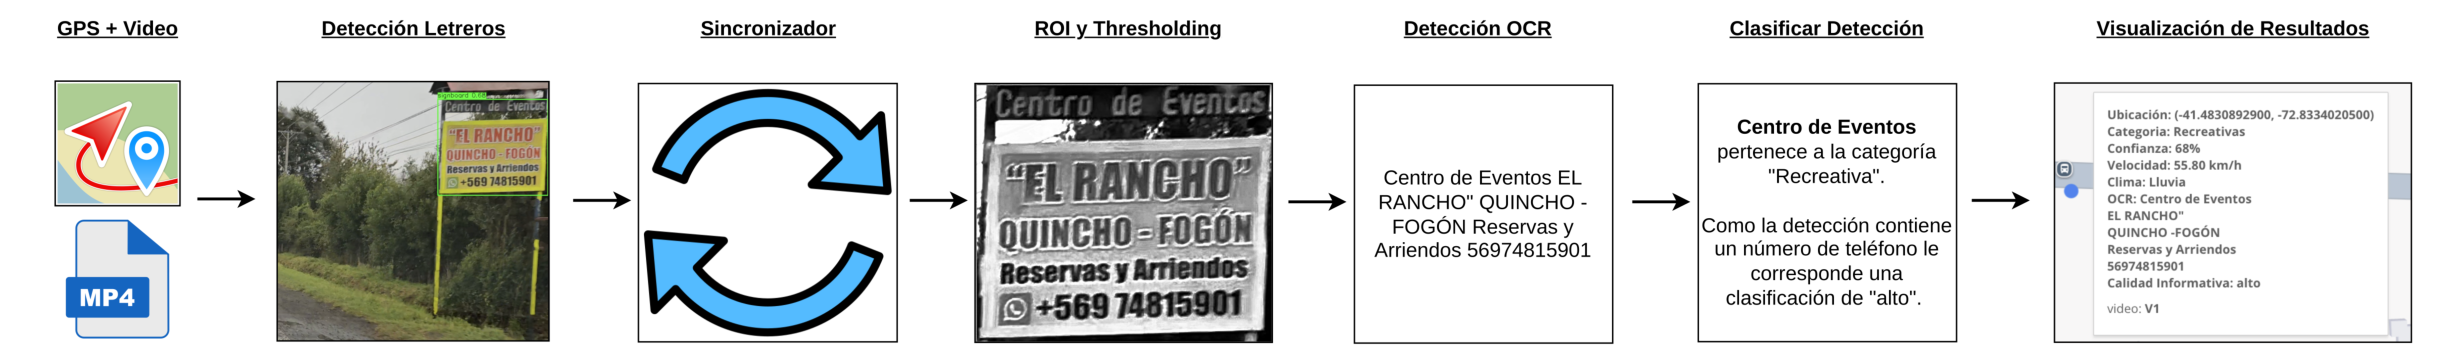
\includegraphics[width=\textwidth]{resultados/pipeline-end-to-end.pdf}
    \caption{Ejemplo end-to-end del pipeline GEODETECTOR sobre un 
    letrero turístico capturado en V1.}
    \label{fig:pipeline_ejemplo}
\end{figure}

A continuación, la Figura~\ref{fig:mapa_resultados} presenta el mapa 
interactivo generado por Google Data Studio \cite{data-studio} para 
el pipeline con las detecciones obtenidas en los tres videos de prueba, 
donde cada punto corresponde a un letrero turístico detectado y 
georreferenciado. Los puntos de color azul, naranja y morado representan
 las detecciones de V1, V2 y V3, respectivamente, permitiendo 
 visualizar la distribución geográfica de la señalética turística a 
 lo largo de las rutas evaluadas en la Región de Los Lagos.

Además, al seleccionar cualquiera de los puntos en el mapa, es 
posible visualizar una tarjeta con información detallada de la 
detección correspondiente. Entre los atributos disponibles se 
incluyen las coordenadas geográficas, la categoría asignada, 
el nivel de confianza de la detección, la velocidad 
registrada durante la captura, las condiciones climáticas, el texto 
extraído mediante OCR y la calidad informativa para el letrero 
detectado.

% con un width de 0.8 se ve mas grande y pasa a la otra pagina
\begin{figure}[H]
    \centering
    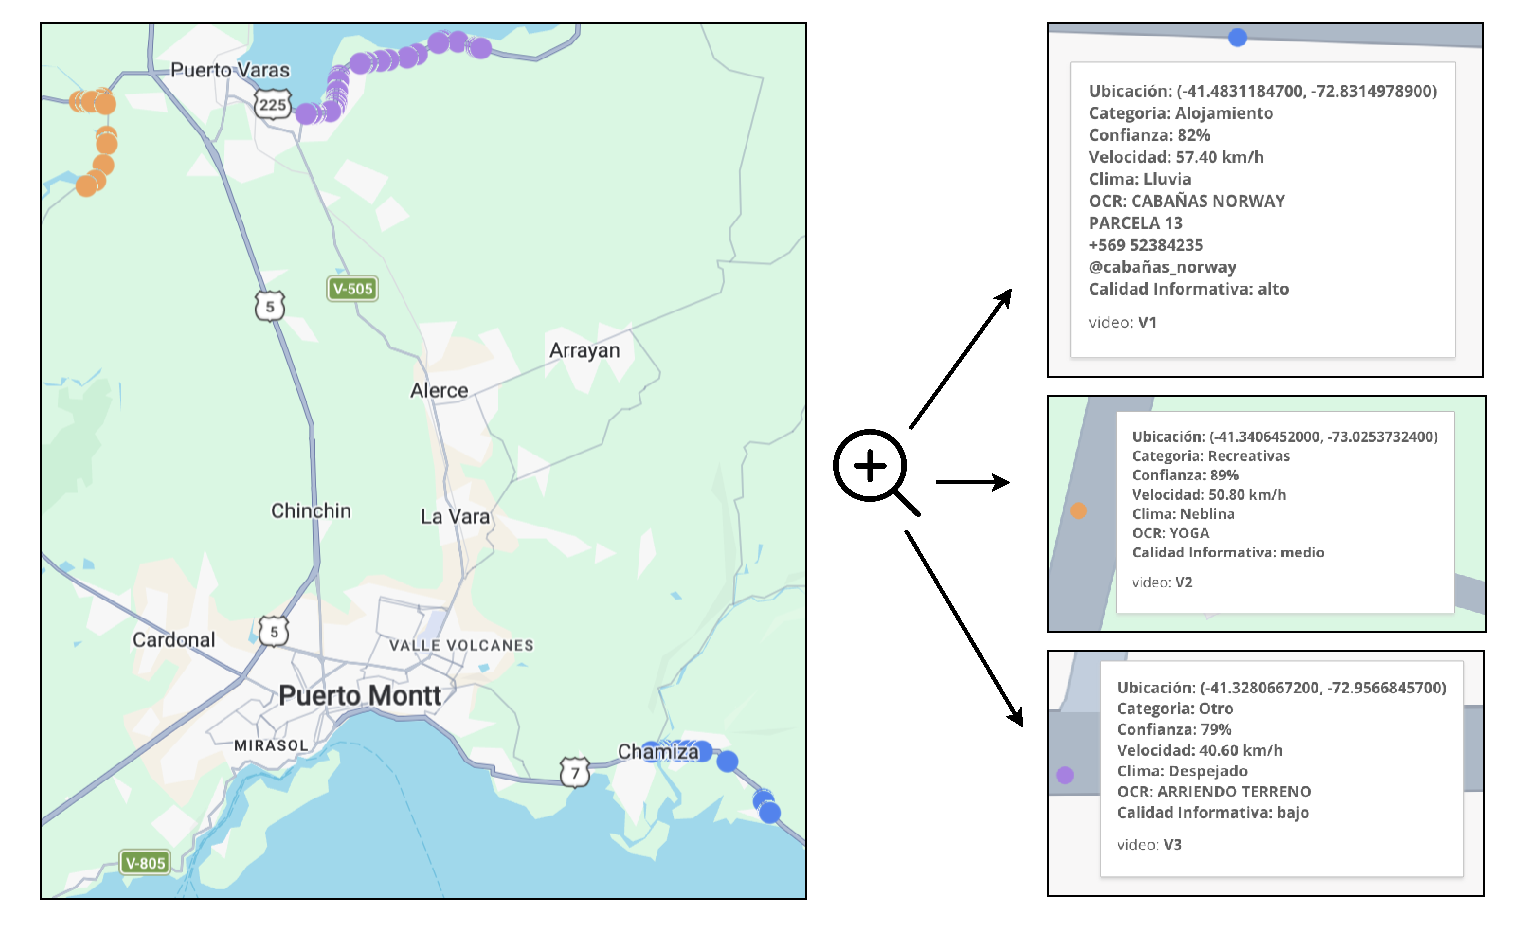
\includegraphics[width=0.8\textwidth]{resultados/mapa-3-videos.pdf}
    \caption{Distribución geográfica de las detecciones obtenidas 
    en los tres videos de prueba.}
    \label{fig:mapa_resultados}
\end{figure}

% =====================================================
\section{Discusión}

Los resultados obtenidos demuestran que el pipeline propuesto es viable para la
 detección y extracción de información desde señalética turística en condiciones reales de captura vehicular. Considerando el promedio de Precisión y Recall 
sobre todas las configuraciones evaluadas, se obtiene una Precisión promedio de 0,84 y un Recall promedio de 0,60. 
La Precisión promedio presenta una diferencia de solo 0,04 respecto al valor obtenido durante el entrenamiento del 
modelo (0,88), lo que indica que el modelo mantiene una alta capacidad para reconocer correctamente los letreros 
en condiciones reales, validando la decisión de entrenar un modelo propio sobre un dataset recolectado en terreno 
en lugar de recurrir a modelos de propósito general que, como se evaluó en las pruebas preliminares, no contemplan 
este tipo de señalética en sus clases predefinidas. El Recall promedio, en cambio, presenta una caída más pronunciada 
respecto al valor de entrenamiento (0,83), diferencia que era esperable considerando que el modelo fue entrenado 
sobre imágenes estáticas en condiciones más controladas, mientras que los videos de prueba introducen desenfoque 
por movimiento (\textit{motion blur}) producto de la velocidad del vehículo, lo que reduce la nitidez de los frames 
y dificulta la detección de letreros que aparecen brevemente en escena.

La degradación progresiva del desempeño en condiciones adversas como 
lluvia y neblina era esperable y está documentada en trabajos previos 
sobre detección en entornos dinámicos \cite{yolo-escenarios-naturales}.
 Esto se refleja en los resultados de detección, donde el Recall oscila entre 0,50 y 0,67 en la mayoría de configuraciones,
indicando que una proporción relevante de letreros no es detectada, 
especialmente a 15 FPS.

Si bien el modelo de detección de letreros demuestra ser preciso y confiable en la 
mayoría de los escenarios evaluados, se observaron casos en que objetos 
de geometría similar a un letrero, como costados planos de camiones, 
banderas o superficies rectangulares en el entorno vial, generaron 
detecciones incorrectas, tal como se observa en la 
Figura~\ref{fig:falsos_positivos}. Asimismo, el modelo reconoce 
ocasionalmente señales de tránsito convencionales que, si bien no 
son de interés para el dominio turístico, comparten características 
visuales con los letreros objetivo, lo cual es atribuible al proceso de 
transfer learning desde pesos preentrenados en dominios viales generales.

\begin{figure}[H]
    \centering
    
    \begin{subfigure}[b]{0.23\textwidth}
        \centering
        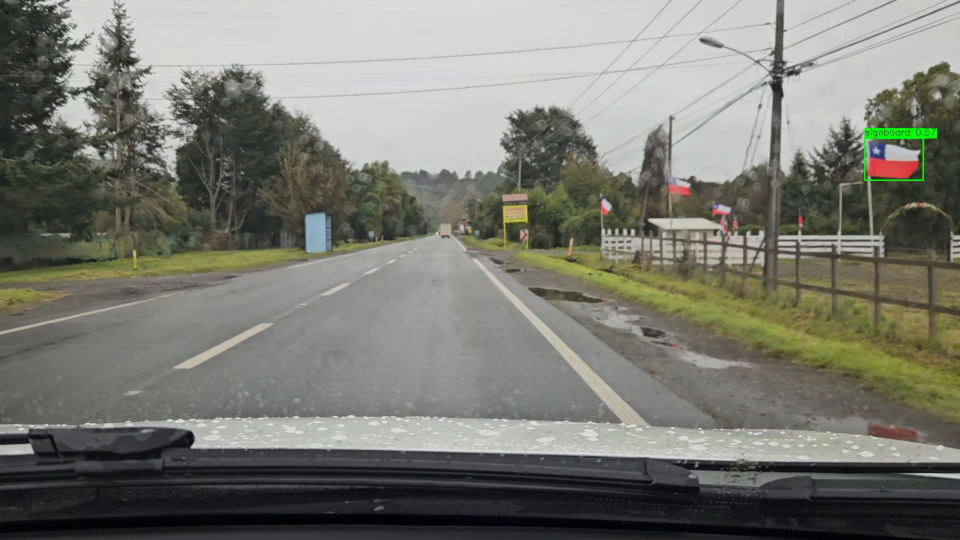
\includegraphics[width=\textwidth]{falsos-positivos/1_comprimido.pdf}
    \end{subfigure}
    \hfill
    \begin{subfigure}[b]{0.23\textwidth}
        \centering
        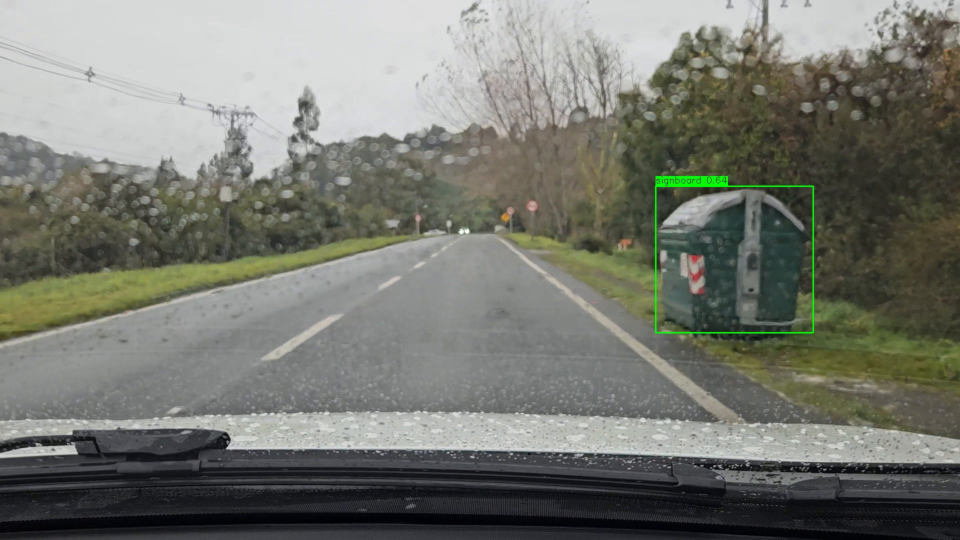
\includegraphics[width=\textwidth]{falsos-positivos/2_comprimido.pdf}
    \end{subfigure}
    \hfill
    \begin{subfigure}[b]{0.23\textwidth}
        \centering
        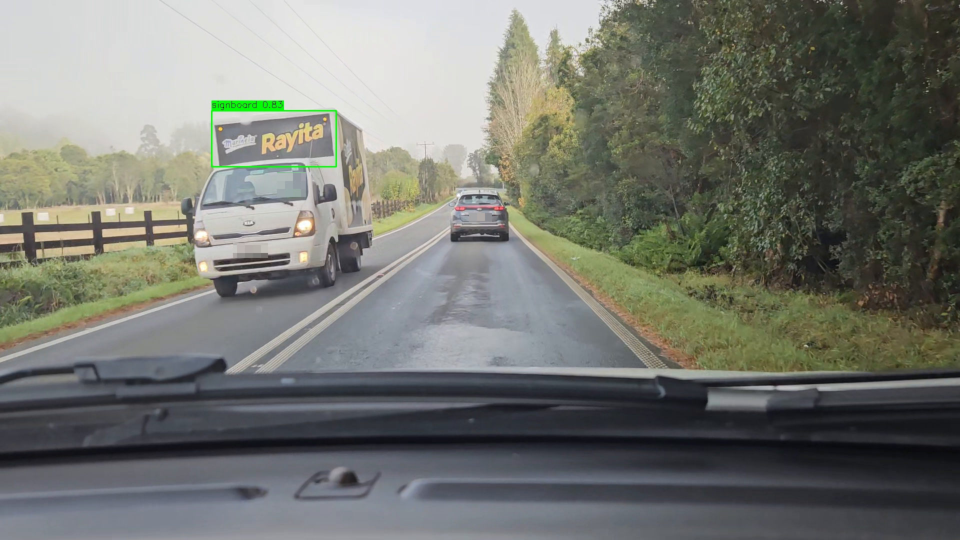
\includegraphics[width=\textwidth]{falsos-positivos/4_comprimido.pdf}
    \end{subfigure}
    \hfill
    \begin{subfigure}[b]{0.23\textwidth}
        \centering
        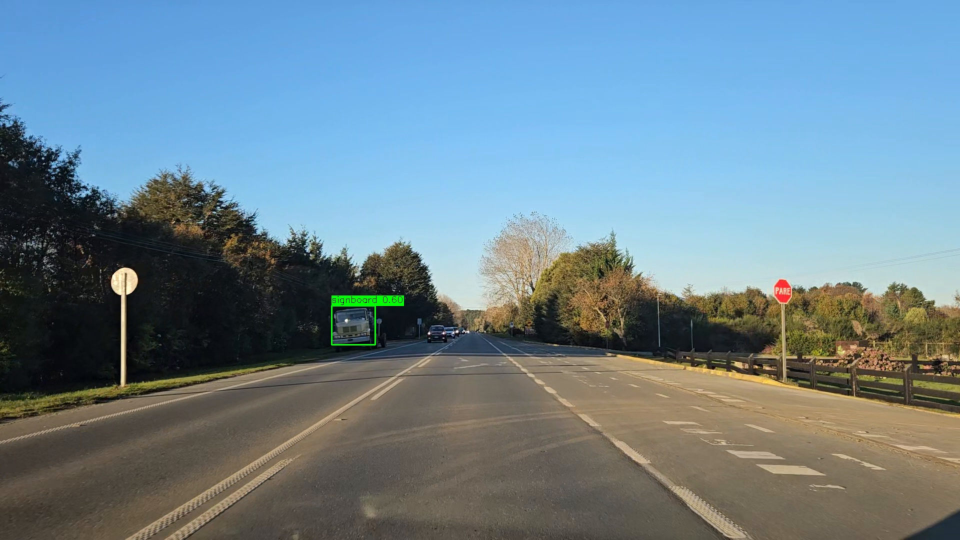
\includegraphics[width=\textwidth]{falsos-positivos/3_comprimido.pdf}
    \end{subfigure}
    
    \caption{Frames con detecciones incorrectas del YOLO11m-customizados (V1, V1, V2 y V3 de izquierda a derecha, respectivamente).}
    \label{fig:falsos_positivos}
\end{figure}

El reconocimiento de texto constituye la etapa de mayor sensibilidad del
pipeline. A diferencia de la detección de letreros, cuyo desempeño depende principalmente
 de la calidad del modelo, el OCR está condicionado por la calidad del frame 
que recibe como entrada, sobre la cual el pipeline no tiene control directo. Factores como el movimiento del vehículo, 
el deterioro físico de los letreros, las condiciones climáticas adversas y la presencia de suciedad o reflejos en el parabrisas
pueden degradar significativamente la nitidez de la imagen capturada, afectando directamente la capacidad del módulo de extraer 
texto de forma confiable. Esta dependencia de la calidad óptica de entrada se refleja en los resultados de CER, donde 
las configuraciones de 15 FPS obtienen consistentemente valores 
deficientes (CER $>$ 0,20) en prácticamente todos los videos, 
mientras que las configuraciones de 30 FPS a 1080p alcanzan valores aceptables o buenos.

Finalmente, la taxonomía de clasificación adoptada (alimentación, alojamiento, recreativa y otros) fue diseñada 
para el dominio turístico, pero la arquitectura del pipeline es extensible a otras categorías. Una variación en la taxonomía 
permitiría identificar, por ejemplo, letreros de venta de terrenos, avisos de servicios agrícolas u otra señalética de interés para distintos casos de uso, 
lo que amplía el alcance potencial del pipeline más allá del turismo.


% =====================================================
\section{Limitaciones}

% dataset, condiciones extremas, OCR
El presente trabajo presenta algunas limitaciones que deben considerarse al
interpretar los resultados. En primer lugar, el dataset de entrenamiento
comprende 2.000 imágenes, las cuales abarcan un conjunto representativo de
escenarios, aunque no incluyen toda la variabilidad existente en cuanto a 
contextos, condiciones climáticas, tipos de letrero y regiones geográficas. 
En consecuencia, el desempeño del modelo podría verse afectado al enfrentarse
a escenarios significativamente diferentes de aquellos presentes durante el
entrenamiento.

En segundo lugar, el pipeline asume condiciones de captura controladas,
considerando un parabrisas en buen estado y limpio (a excepción de V1, donde 
las condiciones de lluvia afectaron la visibilidad), el dispositivo instalado
 en un soporte con un ángulo de captura óptimo y orientación horizontal, tal 
 como se recomienda en la Subsección~\ref{sec:captura}. Variaciones 
 significativas en estas condiciones pueden afectar el desempeño del pipeline.

En tercer lugar, el módulo OCR presenta dificultades ante condiciones extremas
de captura, como velocidades superiores a 80 km/h, letreros muy deteriorados
o ángulos de captura muy pronunciados, escenarios en los que la información
extraída puede ser parcial o incorrecta.

Finalmente, el pipeline no contempla detección nocturna con iluminación artificial, lo que restringe su aplicabilidad a capturas diurnas o en condiciones de luminosidad aceptable.


% =====================================================
\section{Trabajo Futuro}

% mejoras, escalabilidad, edge computing
A partir de los resultados obtenidos y las limitaciones identificadas, 
se plantean las siguientes líneas de trabajo futuro. En primer lugar, 
el pipeline actual opera de forma local y requiere intervención 
técnica para su ejecución, por lo que una mejora natural sería el 
desarrollo de una plataforma web con frontend que permita a un 
administrador cargar el video y el archivo de geolocalización de 
forma autónoma, delegando al pipeline el procesamiento como backend y 
presentando los resultados en una interfaz amigable y accesible para 
usuarios no técnicos.

En segundo lugar, el almacenamiento actual de detecciones y resultados 
debería migrarse hacia un sistema de base de datos, ya sea 
relacional (SQL) o documental (NoSQL), que permita consultas eficientes, 
historial de ejecuciones y escalabilidad ante un mayor volumen de datos.
Esto facilitaría además la integración con otros sistemas de información 
territorial o turística.

En tercer lugar, sería valioso desarrollar una aplicación móvil propia 
bajo el estándar de Progressive Web App (PWA) para la captura y 
registro de geolocalización durante la grabación del video, 
eliminando la dependencia de aplicaciones externas como GeoTracker 
y permitiendo una sincronización más precisa y directa entre el 
flujo de video y los datos GPS.

Finalmente, desde el punto de vista del modelo, se plantea ampliar el 
dataset de entrenamiento con imágenes de regiones geográficas más diversas
para mejorar la capacidad de generalización, así como explorar técnicas 
de mejora de imagen previas al OCR, como super-resolución \cite{ultralytics_super_resolution}
o corrección de desenfoque \cite{correcion-desenfoque}, que permitan reducir el impacto de las condiciones 
adversas sobre la calidad del reconocimiento de texto. En paralelo, 
dado que el área de reconocimiento de texto en escenas naturales es un 
campo en constante evolución, se considera relevante evaluar 
periódicamente nuevos motores OCR que vayan surgiendo en la literatura, 
con el fin de identificar aquel que mejor se ajuste a las condiciones 
particulares del dominio. A largo plazo, la incorporación de capacidades 
de procesamiento en el borde (edge computing) abriría la posibilidad de 
ejecutar el pipeline en tiempo real directamente desde el vehículo, 
sin necesidad de procesamiento posterior.
% =====================================================
\section{Conclusiones}

Este trabajo presentó un pipeline híbrido para la detección, 
reconocimiento de texto, clasificación semántica por taxonomía y 
georreferenciación automática de letreros turísticos en rutas, evaluado 
bajo condiciones reales de captura vehicular. En respuesta a la pregunta 
de investigación \textbf{RQ} planteada, GEODETECTOR demuestra que es 
posible diseñar un pipeline híbrido basado en visión artificial y 
geolocalización capaz de detectar y extraer información relevante desde 
letreros turísticos en condiciones dinámicas no controladas, alcanzando 
valores de Precisión entre $0{,}77$ y $0{,}91$, Recall entre $0{,}50$ 
y $0{,}74$, y F1-score entre $0{,}61$ y $0{,}76$ en los tres videos 
evaluados bajo distintas condiciones climáticas y de resolución (720p 
y 1080p a 15 y 30 FPS). El reconocimiento de texto representa la etapa 
de mayor complejidad del pipeline, dado que el OCR opera sobre frames 
capturados en movimiento en entornos naturales no controlados, 
obteniendo valores de Character Error Rate (CER) entre 0,08 (Bueno) y 
0,27 (Deficiente) dependiendo de la calidad de captura y las condiciones 
presentes en cada video. Adicionalmente, la evaluación end-to-end del 
pipeline en su configuración original (1080p, 30 FPS) reveló que el 
umbral de confianza OCR actúa como un filtro significativo sobre los 
letreros turísticos correctamente detectados: solo el 52,4\%
(11/21) en V1 y el 55,6\% (10/18) en V3 lograron ser 
efectivamente evaluados y clasificados, mientras que en V2 esta 
proporción alcanzó el $100\%$ (3/3), lo que se tradujo en una tasa
 global de evaluación del 57,1\% (24/42).

La contribución de este trabajo es doble: por un lado, 
la construcción de un dataset representativo de señalética 
turística rural capturado en condiciones dinámicas reales, 
ausente en la literatura existente; por otro, el diseño y 
evaluación de un pipeline end-to-end que opera fuera de condiciones 
controladas, aportando evidencia sobre la viabilidad de aplicar visión 
artificial en dominios de alta variabilidad visual. 
Los hallazgos pueden ser de utilidad para organismos de turismo, 
municipios y planificadores territoriales interesados en automatizar 
el inventariado de infraestructura turística vial.

% =====================================================

\section{Agradecimientos}
Quiero agradecer profundamente a mis padres, Claudia y Sebastián, por 
darme la oportunidad de estudiar lejos de casa, por el apoyo incondicional, 
por cada llamada, cada visita y cada gesto de cariño que hizo más 
llevadero este proceso. A mi hermano Bruno, por ser parte de este camino.
¡Lo logramos!

A mi abuelita Ester, por encomendarme siempre al Padre Pancho y por sus 
oraciones que sin duda llegaron lejos. Agradezco a Dios por tenerla 
aquí, con 94 años, con su salud y su alegría, pudiendo vivir este logro 
juntos. A mi abuelita Gladys, por sus llamadas, sus regalos y su cariño 
constante. A mi madrina Carmen, mi padrino Jorge, mis tías Cholita, 
Lucy y Tina, y mi tío Jorge, por sus buenos deseos y el cariño que me 
han dado siempre.

Quiero enviar un saludo especial al cielo, a quienes ya no están hoy, 
pero estoy seguro de que estarían felices con este logro: Kokito, 
Abuelita Irene, Tía Juanita, Tía Lili, Tía Marlene, Tío Aldo y 
Miguelito. ¡Abrazos al cielo, esto es para ustedes también! Y a nuestra 
primera mascota, Clarita Belén, que descansa en el cielo animal, 
gracias por haber sido parte de nuestra familia.

Se agradece al profesor patrocinante Luis Veas por proponer un tema de 
tesis tan interesante y enriquecedor, alineado con mis áreas de interés, 
que fue un verdadero gusto desarrollar. Sus indicaciones, revisiones, 
comentarios y correcciones fueron fundamentales para guiar y mejorar 
este trabajo a lo largo de todo el proceso, y al profesor 
co-patrocinante Christian Lazo por su apoyo en la publicación del 
dataset en IEEE DataPort. Se agradece también a Javier Reyes y Handel 
Venegas por su colaboración en el proceso de etiquetado manual del dataset.

Se agradece a Carlos Duarte por su ayuda en la instalación de 
contenedores, librerías y herramientas necesarias para el entorno de 
trabajo y su apoyo para aprender a utilizar el supercomputador 
Patagón UACh, y al profesor Cristóbal Navarro, administrador de dicho 
supercomputador, por facilitar el acceso a los recursos de cómputo 
fundamentales para el desarrollo de esta investigación y por su 
disposición para resolver dudas técnicas relacionadas con el entorno 
de trabajo.

Esta investigación fue apoyada por el supercomputador Patagón de la 
Universidad Austral de Chile (FONDEQUIP EQM180042).

Finalmente, un agradecimiento a los amigos que conocí en esta etapa 
y que hicieron de estos años universitarios una experiencia 
inolvidable: Tomás, Renato, Handel, Javier, Fernando C., Fernando I., 
Vicente, Luciano y Francisco.



\bibliographystyle{plain}
\bibliography{sample}


\end{document}